\documentclass[12pt,spanish,chapterprefix, numbers=noenddot]{book}
\usepackage{amsmath}
\usepackage{amsthm}
\usepackage{fontspec}
\usepackage[a4paper]{geometry}
\geometry{verbose,tmargin=2.5cm,bmargin=2.5cm,lmargin=2.5cm,rmargin=2.5cm,headheight=1cm,headsep=1cm,footskip=1cm}
\setlength{\parskip}{\medskipamount}
\setlength{\parindent}{0pt}
\usepackage{color}
\usepackage{babel}
\addto\shorthandsspanish{\spanishdeactivate{~<>}}

\usepackage{float}
\usepackage{makeidx}
\makeindex
\usepackage{graphicx}
\usepackage{nomencl}
% the following is useful when we have the old nomencl.sty package
\providecommand{\printnomenclature}{\printglossary}
\providecommand{\makenomenclature}{\makeglossary}
\makenomenclature
\usepackage[unicode=true,pdfusetitle,
 bookmarks=true,bookmarksnumbered=false,bookmarksopen=false,
 breaklinks=true,pdfborder={0 0 0},pdfborderstyle={},backref=false,colorlinks=true]{hyperref}
\hypersetup{
 allcolors=blue}
\usepackage{listings}
\makeatletter

%%%%%%%%%%%%%%%%%%%%%%%%%%%%%% LyX specific LaTeX commands.
\newcommand{\noun}[1]{\textsc{#1}}
\providecommand\textquotedblplain{%
  \bgroup\addfontfeatures{Mapping=}\char34\egroup}
%% Because html converters don't know tabularnewline
\providecommand{\tabularnewline}{\\}
\floatstyle{ruled}
\newfloat{algorithm}{tbp}{loa}[chapter]
\providecommand{\algorithmname}{Algoritmo}
\floatname{algorithm}{\protect\algorithmname}

%%%%%%%%%%%%%%%%%%%%%%%%%%%%%% Textclass specific LaTeX commands.
\numberwithin{equation}{section}
\numberwithin{figure}{section}
\providecommand*{\code}[1]{\texttt{#1}}

%%%%%%%%%%%%%%%%%%%%%%%%%%%%%% User specified LaTeX commands.
%Para que las URLs de la bibliografía se pueda pinchar
\usepackage{url}

%Cabeceras y pies de página
\usepackage{fancyhdr}
\pagestyle{fancy}
\lhead[\rightmark]{}
\rhead[]{\leftmark}
\cfoot{\thepage}

%Para que los índices respeten los espacios de las nuemraciones
\usepackage[tocindentauto]{tocstyle}
\usetocstyle{standard}

%Para que ponga "Índice de Tablas" en vez de "Indice de Cuadros"
\addto\captionsspanish{
\def\tablename{Tabla}
\def\listtablename{\'Indice de tablas}
}

%Para que las páginas en blanco no tengan cabecera ni número de página
\makeatletter
\renewcommand*{\cleardoublepage}{\clearpage\if@twoside \ifodd\c@page\else
\hbox{}%
\thispagestyle{empty}%
\newpage%
\if@twocolumn\hbox{}\newpage\fi\fi\fi}
\makeatother



\usepackage{chngcntr}
\counterwithout{figure}{chapter}
\counterwithout{figure}{section}
\counterwithout{table}{chapter}
\counterwithout{algorithm}{chapter}

\setcounter{tocdepth}{3}

\AtBeginDocument{
  \def\labelitemii{\(\circ\)}
  \def\labelitemiii{\(\triangleright\)}
}

\makeatother

\usepackage{listings}
\lstset{basicstyle={\ttfamily},
breaklines=true}
\usepackage[style=numeric,backref=true]{biblatex}
\def\eqdeclaration#1{, véase la ecuación\nobreakspace(#1)}
\def\pagedeclaration#1{, página\nobreakspace#1}
\def\nomname{Nomenclatura}
\renewcommand{\lstlistingname}{Listado de código}

\addbibresource{./refs.bib}
\begin{document}
\frontmatter

\begin{titlepage}

\begin{center}

\includegraphics[width=8cm]{Figs/logoURJC}
\par\end{center}

\begin{center}
Escuela Técnica Superior de Ingeniería de Telecomunicación
\par\end{center}

\vspace{4cm}

\begin{center}
{\LARGE{}MOVIMIENTO PLANIFICADO DE UN BRAZO ROBÓTICO 
EN EL ENTORNO EDUCATIVO ROBOTICS-ACADEMY}{\LARGE\par}
\par\end{center}

\vspace{4cm}

\begin{center}
{\large{}Memoria del Trabajo Fin de Grado}{\large\par}
\par\end{center}

\begin{center}
{\large{}en Ingeniería en Sistemas Audiovisuales y Multimedia}{\large\par}
\par\end{center}

\vspace{4cm}

\begin{center}
{\large{}Autor: Ignacio Malo Segura}{\large\par}
\par\end{center}

\begin{center}
{\large{}Tutor: José María Cañas Plaza}{\large\par}
\par\end{center}

\begin{center}
{\large{}Co-tutor: José Francisco Vélez Serrano}{\large\par}
\par\end{center}

\begin{center}
2019
\par\end{center}

\end{titlepage}

\chapter*{Agradecimientos}

\chapter*{Resumen}
El nuevo período de esplendor tecnológico que se está desarrollando en los últimos años, supone un reto para los ingenieros de cada una de las áreas en crecimiento. Una de ellas es la robótica, que se encarga de utilizar la informática, la mecánica y la electrónica para desarrollar máquinas al servicio de las personas. 

Hoy en día encontramos robots tanto a nivel industrial como doméstico, desde fabricación, coches autónomos o aplicaciones médicas hasta aspiradoras inteligentes o drones. A pesar de ello, la demanda de empleo en las próximas décadas no será satisfecha si se mantienen las previsiones sobre estudiantes en materias de perfil tecnológico. Ante esta situación cobra vital importancia la educación, que debe ser de calidad y accesible para garantizar el futuro de los profesionales que diseñan robots. 

Este proyecto está dirigido a ampliar los recursos de Robotics-Academy, una plataforma que acerca a los estudiantes al software de control de robots a través de prácticas simplificadas, de manera que tomar contacto con la robótica no se convierta en una odisea. Estas prácticas parten de plantillas donde completar la solución a través de código, y permiten resolver algunos problemas típicos de este campo de conocimiento. 

Con este Trabajo de Fin de Grado se ha creado una nueva práctica, utilizando el lenguaje de programación Python, enfocada a conocer la planificación y ejecución de trayectorias con un brazo robótico en un entorno simulado en Gazebo. Para ello, se hace uso de tecnologías extendidas como la librería OpenCV, para el procesado de las imágenes recibidas por el robot, o el \textit{framework} MoveIt!, que ofrece todas las herramientas necesarias para trabajar con robots sobre ROS. El objetivo es conseguir detectar objetos de color, además de planificar y ejecutar movimientos en entornos con obstáculos. 

Este trabajo permite acceder a los distintos recursos a través de interfaces sencillas para trabajar con imágenes y movimientos, abstrayendo al receptor de la misma de detalles de bajo nivel y configuraciones complejas. La experimentación realizada ha permitido profundizar en la planificación hasta lograr unos resultados estables, que serán presentados a continuación.  

\tableofcontents{}

\mainmatter

\chapter{Introducción}
Antes de comenzar a profundizar en un proyecto de robótica es necesario comprender el contexto en el que se sitúa, así como el estado actual de su campo de estudio. A continuación se analizará el porqué del crecimiento que ha experimentado en los últimos años, para después comprender cómo se desarrolla software en robótica y terminar mostrando el funcionamiento de la docencia en esta disciplina a través del entorno Robotics-Academy, al que va dirigido este Trabajo de Fin de Grado. 

\section{Robótica}
La Real Academia Española define la robótica como la "técnica que aplica la informática al diseño y empleo de aparatos que, en sustitución de personas, realizan operaciones o trabajos, por lo general en instalaciones industriales". De aquí se sacan dos ideas principales; trabajar en este área consiste en diseñar y utilizar robots a través de código, y además está enfocada, en un principio, a realizar autónomamente tareas que realizan las personas.

El desarrollo de software para robótica exige controlar cada detalle, teniendo en cuenta también el componente ético que requiere el desarrollo de tecnología. Isaac Asimov, uno de los escritores de ciencia ficción más relevantes de nuestra historia, también pasó a formar parte de la historia de la robótica al enunciar sus tres leyes fundamentales, que sin duda seguirán teniéndose muy en cuenta ahora que los robots son una realidad:
\begin{itemize}
    \item Un robot no hará daño a un ser humano o, por inacción, permitirá que un ser humano sufra daño
    \item Un robot debe obedecer las órdenes dadas por los seres humanos excepto si estas órdenes entrasen en conflicto con la 1ª ley.
    \item Un robot debe proteger su propia existencia en la medida en que esta protección no entre en conflicto con la 1ª o la 2ª Ley.
\end{itemize}

Para entender completamente la importancia del tema expuesto, conviene asimilarlo a sucesos históricos previos. El ser humano, a lo largo de su historia, se ha caracterizado por su afán de superación, y esa necesidad por obtener más es la que le ha llevado a la excelencia en muchos aspectos tecnológicos. 

Si nos remontamos a la segunda mitad del siglo XVIII,  nos encontramos con una serie de cambios en la tecnología, la sociedad y la cultura que propiciaron la Revolución Industrial. Ésta supuso uno de los grandes saltos cualitativos en cuanto al progreso humano, al centrar las actividades de trabajo en procesos que utilizaban máquinas en sustitución de tareas manuales. Ello llevó principalmente a un incremento de la producción, de la mano de una mejora en el transporte a raíz del uso de la máquina de vapor, a costa de algunos conflictos sociales o el inicio del agotamiento de recursos energéticos y el incremento de la contaminación. 

A finales del siglo XIX y comienzos del XX, nos encontramos con una serie de descubrimientos y nuevos recursos, como el petróleo o la electricidad, que aceleraron enormemente el crecimiento industrial y permitieron mejorar la calidad del transporte. Estos, juntos a los avances científicos supusieron una mejora de la calidad de vida de las personas.

El siguiente gran salto tecnológico es el más cercano en el tiempo y, sin duda, es el que propicia la posterior aparición de los robots. Los descubrimientos de la segunda mitad del siglo XX en el campo de la electrónica, causaron la explosión de la informática y las telecomunicaciones, desencadenando transformaciones sociales, culturales y económicas tan importantes como las que provocó la llegada de Internet. La concienciación para el uso de las energías renovables o la aparición de nuevas tecnologías de la información y la comunicación son otros aspectos destacables. 

Si se observa el imparable crecimiento del porcentaje de usuarios de Internet en el mundo desde 1990 hasta la actualidad (ver Figura \ref{fig:internetWorldwide}), donde ya es superior al 50\% de los individuos, es fácil hacerse una idea de la influencia que ha alcanzado en todos los niveles de la sociedad. Pero no está todo hecho ya que, como se comenta al inicio del razonamiento, el ser humano quiere, puede, y debe seguir progresando tecnológicamente.  %pending: unificar figuras en todo el doc

\begin{figure}[hbt!]
\centering
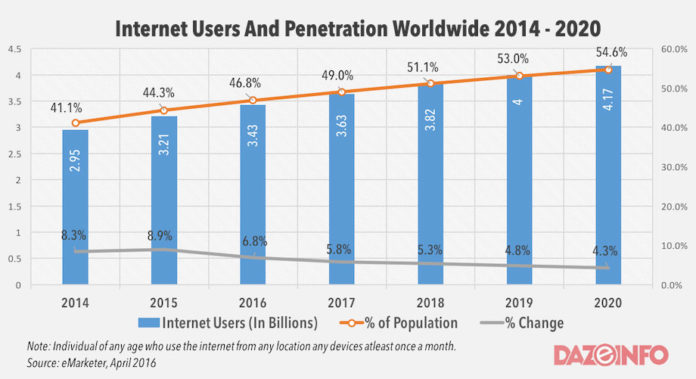
\includegraphics[width=12cm]{Figs/internetWorldwide.jpg}
\par
\caption{\label{fig:internetWorldwide}Predicción del número de usuarios en Internet 2016-2020}
\end{figure}

En el Foro Económico Mundial de 2016 
\cite{forum_2016} apareció el término Cuarta Revolución Industrial para referirse al siguiente movimiento de esplendor tecnológico: nanotecnología, inteligencia artificial, robótica, computación en la nube, big data, biotecnología, vehículos autónomos, nuevos sistemas de almacenamiento de energía, nuevos materiales, impresión 3D. Sin duda es un reto apasionante para los ingenieros y profesionales de cada una de las áreas de conocimiento, algo posible gracias a un cúmulo de avances a lo largo de los siglos y que ahora es el momento de continuar. 


\subsection{El sector: presente y futuro}
Hoy los robots son una realidad. No sólamente son utilizadas por importantes empresas en labores industriales, como Tesla en la fabricación de vehículos o Amazon en la gestión de almacenes. La NASA utiliza robots para sus misiones espaciales, como el Curiosity para la exploración de la superficie de Marte.  En el ámbito militar, el robot TEODOR permite evitar situaciones de alto riesgo para los humanos como la desactivación de explosivos. En la medicina, Da Vinci permite al cirujano operar a través de una consola para mejorar la precisión y reducir riesgos en ciertas operaciones quirúrgicas. Además, han ido adquiriendo importancia gradualmente en los hogares y la vida cotidiana de las personas. Desde robots aspiradores que reconocen el entorno, lo memorizan y limpian la casa periódicamente, hasta los avances que encaminan a los vehículos hacia la conducción autónoma. 

El mercado de la robótica está llamado a convertirse en uno de los más importantes del presente siglo, alcanzando una valoración estimada superior a los 28 billones de euros en el año 2018 \cite{robotics_market}. En los últimos años ha experimentado un gran crecimiento y se espera que continúe en los próximos años, con una previsión de un 25\% de revalorización para los próximos 5 años. 
Una posible explicación para este hecho se fundamentaría en la aún reciente tendencia a la automatización de tareas a nivel empresarial, sumado en menor medida a un incremento en la compra de tecnología robótica a nivel usuario.

Ahora bien, ¿cuáles son las razones que explican este crecimiento de la automatización, y hacia dónde nos lleva?. Aunque hay algunas características propias del ser humano, como la creatividad o la impredecibilidad, que son imposibles de reemplazar hasta el momento, algunas de las razones que explican las tendencias comentadas son:
\begin{itemize}
\item Aumento de la eficiencia 
\item Productividad sin descanso
\item Reducción de costes
\item Evita el error humano
\item Más precisión
\item Control de errores
\end{itemize}
Por otro lado, uno de los factores clave para comprender el futuro del sector es el impacto que puede tener en el mercado laboral tal y como lo conocemos actualmente. Algunos estudios \cite{automation_forecast} \cite{mckinsey_automation} apuntan que dentro de 35 años, más del 50\% de los trabajos estarán automatizados, con el impacto que eso conlleva para los diferentes trabajadores, que podrían perder puestos de trabajo en favor de profesionales del software que serán necesarios para afrontar el proceso de transición, y posterior mantenimiento de esta digitalización. 

Los perfiles STEM (carreras relacionadas con ciencia, tecnología, ingeniería y matemáticas) van a ser cada vez más demandados en los próximos años, con el hándicap de que el número de nuevos profesionales relacionados con estas áreas disminuye cada año. 
Si vemos los datos de empleos relacionados con alta tecnología (ver Figura \ref{fig:empleoEur}) en nuestro país, y los comparamos con el resto de países europeos, observamos que el porcentaje de empleos de este tipo es muy pobre en la gran mayoría de regiones españolas, a excepción de Madrid y, en menor medida, la zona noreste de la península. 

\begin{figure}[hbt!]
\centering
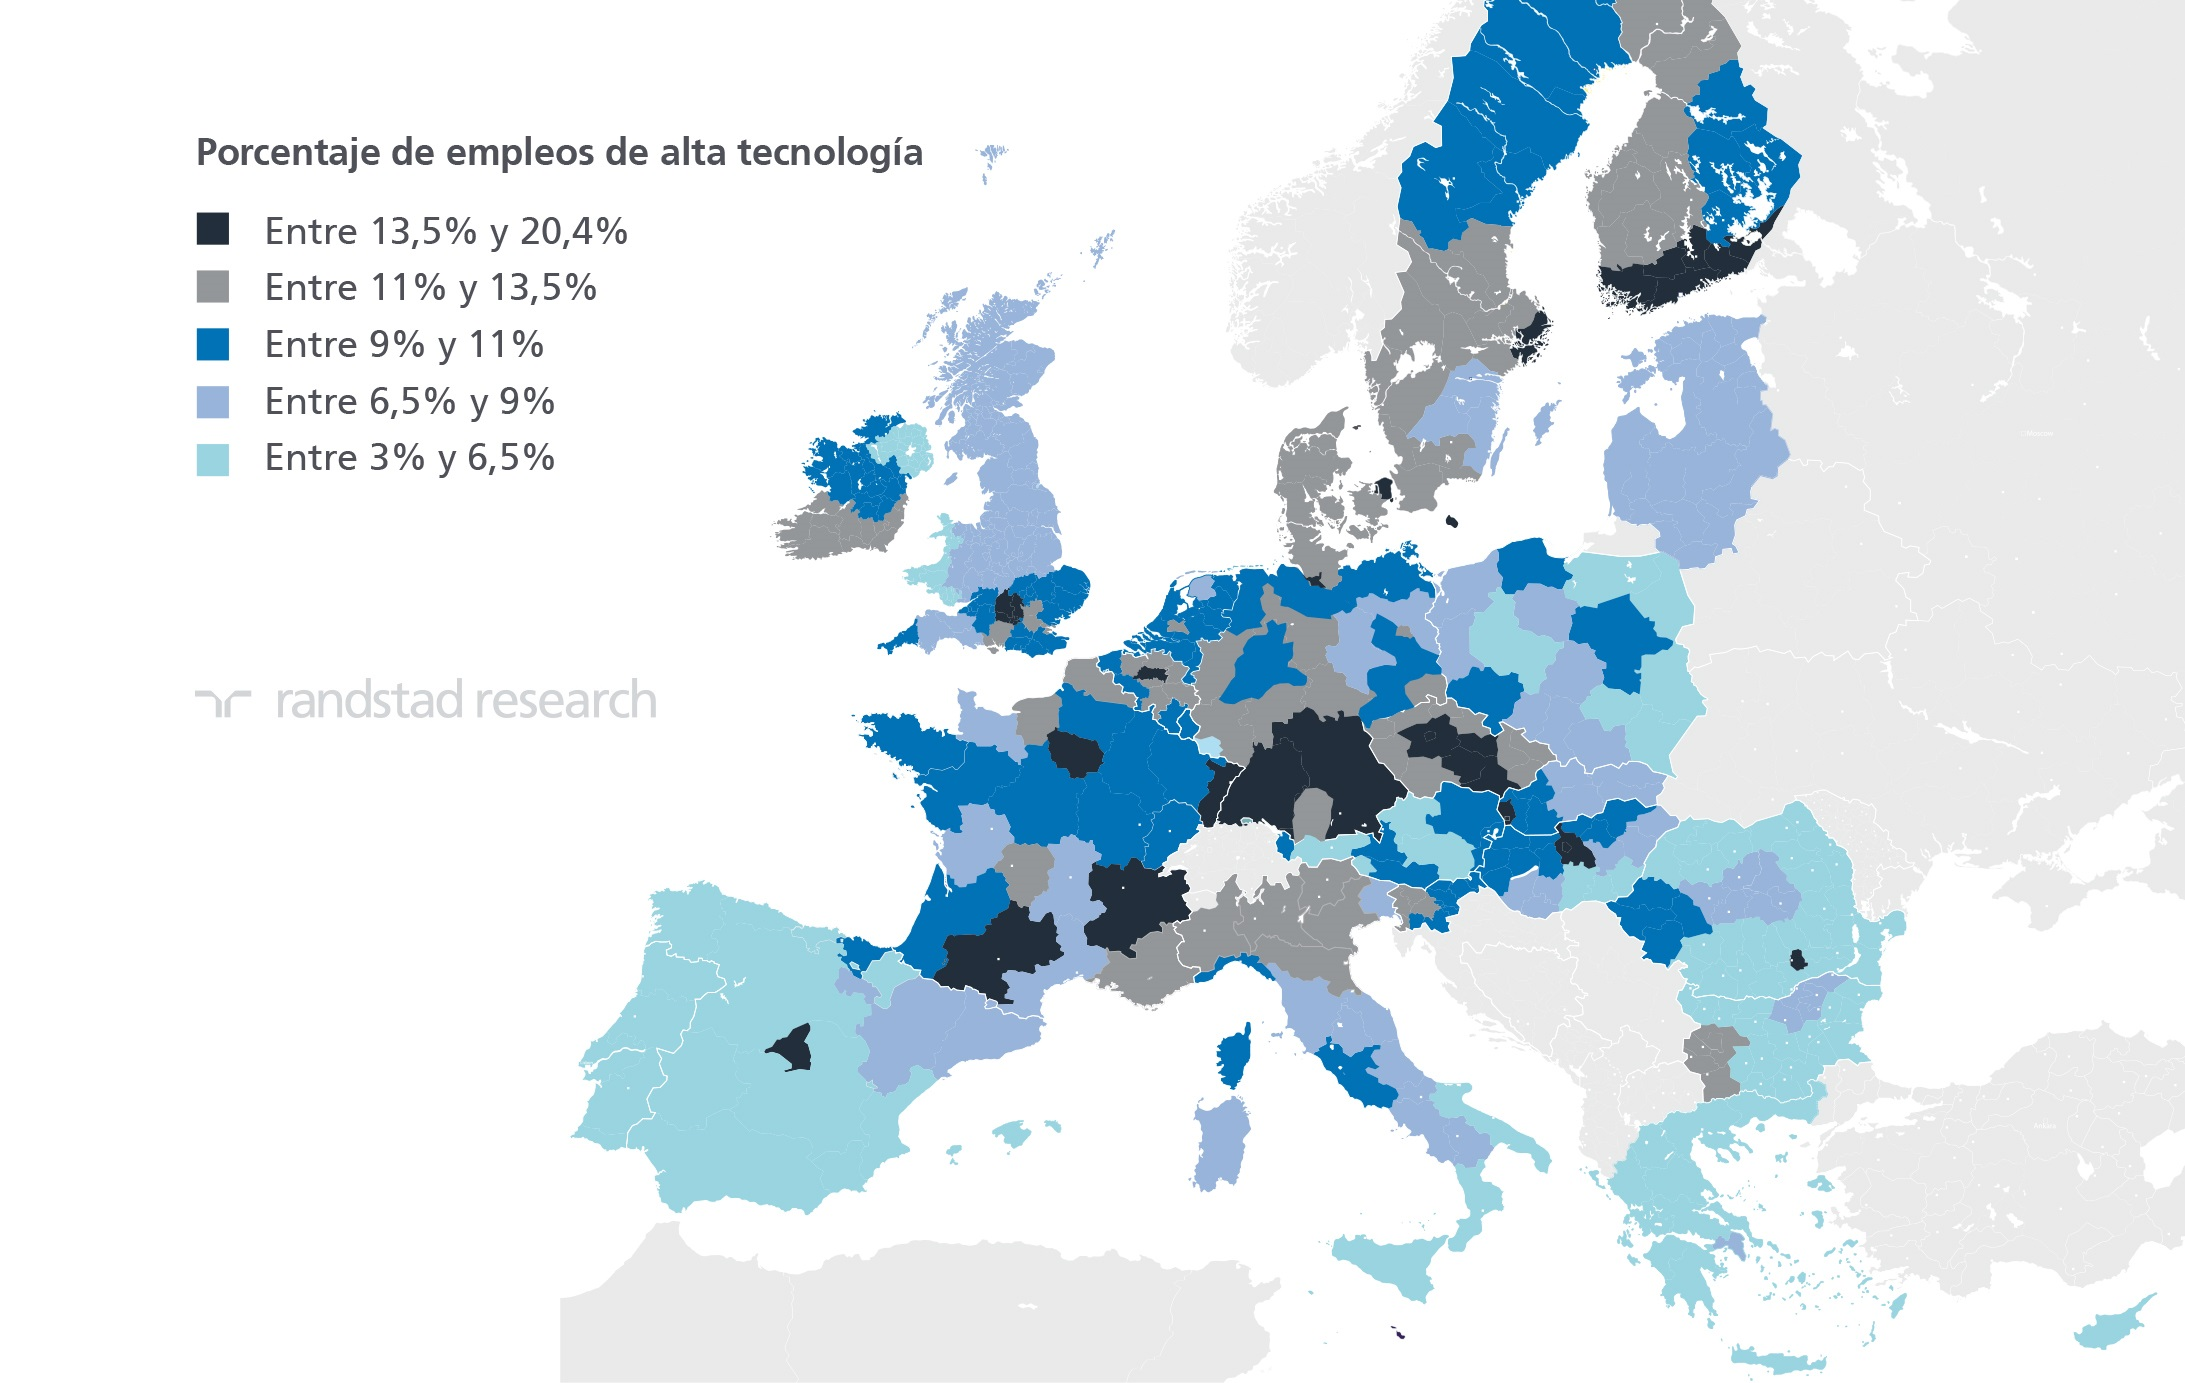
\includegraphics[width=12cm]{Figs/empleosTecEur.jpg}
\par
\caption{\label{fig:empleoEur}Empleos de alta tecnología en Europa}
\end{figure}

\section{Software en robótica}

Lograr el comportamiento esperado en un sistema robótico requiere conocer las distintas partes de las que se compone. Construir un robot supone la interacción de muchos componentes entre sí, formados a su vez por piezas más pequeñas. Entre ellos se encuentran los sensores, los actuadores y el computador. 

En primer lugar, es necesario poder obtener información del entorno a través de la medición de diversas magnitudes físicas. Los sensores deben estar diseñados para obtener las más adecuadas para la tarea a realizar. Las cámaras, sensores láser, sensores de temperatura, de posición o de aceleración son algunos ejemplos. 

La percepción de lo que hay alrededor requiere procesar esos datos mediante un computador para que sean útiles, es decir, se tomen decisiones y se den órdenes a los actuadores, que son los componentes encargados de interacturar con el mundo a través del movimiento. 

El software constituye por tanto el elemento fundamental del robot, dotándolo de inteligencia y determinando su comportamiento. Para lograrlo de una manera adecuada, es necesario adaptarse a algunos requisitos. En primer lugar, el hecho de interactuar con un mundo, el real, que se encuentra en constante movimiento, requiere sistemas que respondan en tiempo real a dichos cambios. Para ello, se requiere hacer uso de la concurrencia para poder tomar decisiones con la mayor rapidez posible, algo crítico teniendo en cuenta la necesaria comunicación entre los distintos componentes. 

De cara al usuario, es necesario construir interfaces que faciliten la interacción con los robots y la depuración de los diferentes problemas que puedan surgir. Estos pueden estar derivados por el hecho de tener que adaptar los programas al hardware heterogéneo existente, o la dificultad que presenta la reutilización de software de fuentes externas. 

Actualmente, la implementación del comportamiento de los robots se realiza mediante software de control. En este contexto de desarrollo es muy útil un entorno que facilite la gran complejidad a la que se enfrenta el ingeniero. En informática, se denomina \textit{middleware} a un software que hace de enlace entre el sistema operativo y las aplicaciones (ver Figura \ref{fig:middleware}). En robótica, este software está diseñado para ocultar parte de la complejidad de bajo nivel, como la comunicación entre los distintos componentes. Así, el desarrollador puede diseñar y desarrollar sus soluciones de forma más eficiente. EN los siguientes párrafos se presentan algunos de los \textit{middlewares} más importantes, y sus principales objetivos: 
\begin{figure}[hbt!]
\centering
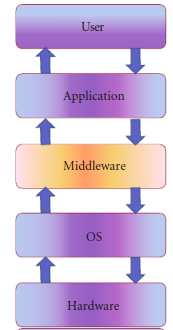
\includegraphics[width=6cm]{Figs/layersMiddleware.png}
\par
\caption{\label{fig:middleware}Situación del \textit{middleware} en una arquitectura software}
\end{figure}
\begin{itemize}
\item ROS \cite{ros}: Robot Operating System continua creciendo hacia su objetivo de ser un estándar en la industria. Se trata de una solución de código abierto. Ofrece robustez, rapidez, abstracción, colaboración entre usuarios y una gran variedad de paquetes y funcionalidades, facilitando la labor de desarrollo. Se estima que en los próximos años supere el umbral y más del 50\% de los robots comerciales estén basados en él. 
\item Orocos \cite{orocos}: Open Robot Control Software centra sus esfuerzos en ofrecer resultados en tiempo real y enfocado principalmente en robots industriales. Para ofrecer algunas funcionalidades, se apoya en otros \textit{middleware}s similares. Es multiplataforma.  
\item CLARAty \cite{claraty}: Promueve la reutilización de software, además de la portabilidad, modularidad y flexibilidad. Surge de la colaboración entre varias instituciones, entre ellas la NASA.
\item MRDS \cite{mrds}: Microsoft Robotics Developer Studio fue el primer intento de la compañía estadounidense por entrar de lleno en el mundo de la robótica. Su lanzamiento se produjo poco antes que el de ROS, por lo que nunca ganó suficiente atención. 
\end{itemize}

\section{Docencia en robótica}
En un mundo necesitado de profesionales de la tecnología, pero cuyos individuos no van a cubrir la demanda de empleos en los próximos años, es necesario hacer accesible el conocimiento. Aquí es donde la docencia, en cualquiera de sus formas, cobra vital importancia. A continuación se comentarán algunos aspectos relacionados con la enseñanza en robótica en la actualidad. 
\subsection{Robótica en la escuela}
Los conocimientos de robótica y programación han estado, hasta fechas muy recientes, alejados de las escuelas, donde aún su influencia es aún limitada. En las universidades,  la robótica está presente solamente en algunas carreras especializadas. Ahora bien, ¿cómo es posible que herramientas básicas para un importante porcentaje de los empleos que vienen en los próximos años hayan comenzado a implantarse hace tan poco tiempo?  \cite{noticia_estudiantes}. Es una pregunta compleja en la que influyen muchos factores, aunque podemos afirmar que algunos de ellos se derivan del hecho de estar hablando de un área de conocimiento joven. Otros factores pueden deberse a la necesidad de cambios legislativos, a necesitar unas bases de conocimiento sólidas en el profesorado, y probablemente un presupuesto superior a otras áreas de enseñanza. 

Si tenemos en cuenta que los futuros profesionales están hoy en las aulas, es necesario mostrar la robótica de una manera cercana, comprensible y que permita generar entusiasmo en los alumnos interesados. Al fin y al cabo, las decisiones que se toman en las últimas etapas de estudios previos a la universidad, son claves para decidir el futuro, y para hacerlo con criterio el alumno necesita el mayor abanico de conocimiento y opciones posible. 
La robótica educativa debe ser más relevante en los próximos años si se quieren formar y educar profesionales para la Cuarta Revolución Industrial. Entre las competencias que aporta al alumnado, están algunas tan necesarias para otros aspectos profesionales y vitales como el trabajo en equipo, el pensamiento crítico, la creatividad y la resolución de problemas. Existen algunas empresas que tratan de facilitar esta tarea ofreciendo robots educativos. Por ejemplo: 
\begin{itemize}
    \item Sphero SPRK+: Enfocada a los más pequeños, programable desde aplicaciones móviles a través de bloques, permite planificar rutas para la bola inteligente. Tiene un diseño transparente para poder ver y aprender de su interior (ver Figura \ref{fig:sphero}).  
    \item Dash: Solución para niños basada en programación con bloques y ampliable con accesorios 
    \item Zowi: La propuesta educativa de BQ tiene su propia interfaz para la programación por bloques, llamada Bitbloq (ver Figura \ref{fig:bitbloq}). La app para controlar el robot tiene como objetivo demostrar que se puede aprender jugando.
    \item Mindstorms: La línea de LEGO dedicada a construir robots a partir de sus míticas piezas (ver Figura \ref{fig:sphero}), permite después aprender a programarlos a través de bloques para que realicen diversas acciones. 
    \begin{figure}[h!]
    \centering
    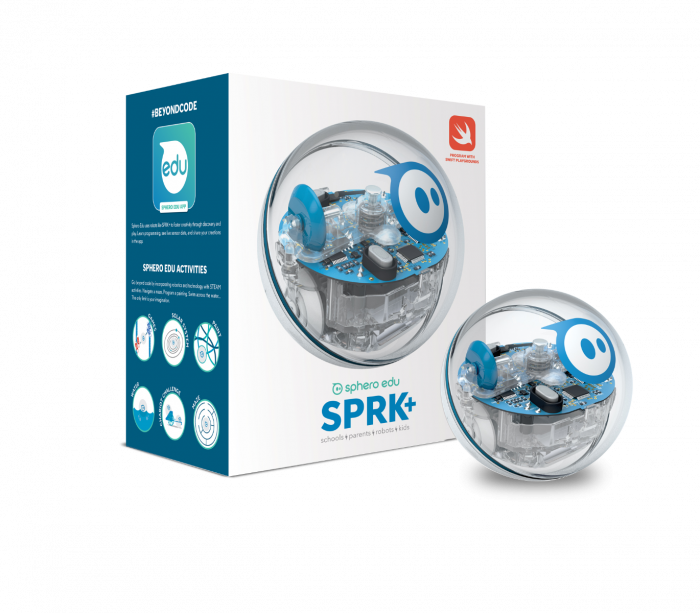
\includegraphics[width=6cm]{Figs/spheroedu-sprkplus.png}
    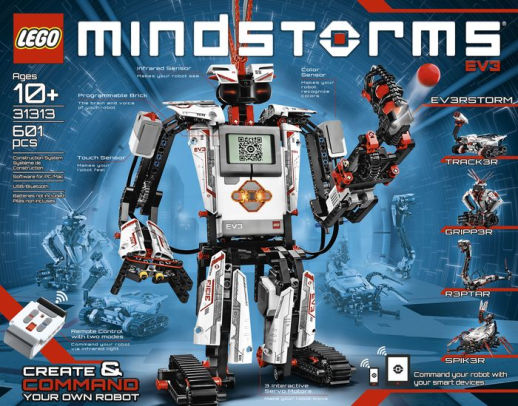
\includegraphics[width=6cm]{Figs/mindstorms.jpg}
    \par
    \caption{\label{fig:sphero}Sphero SPRK+ y LEGO mindstorms}
    \end{figure}
\end{itemize}
    \begin{figure}[h!]
    \centering
    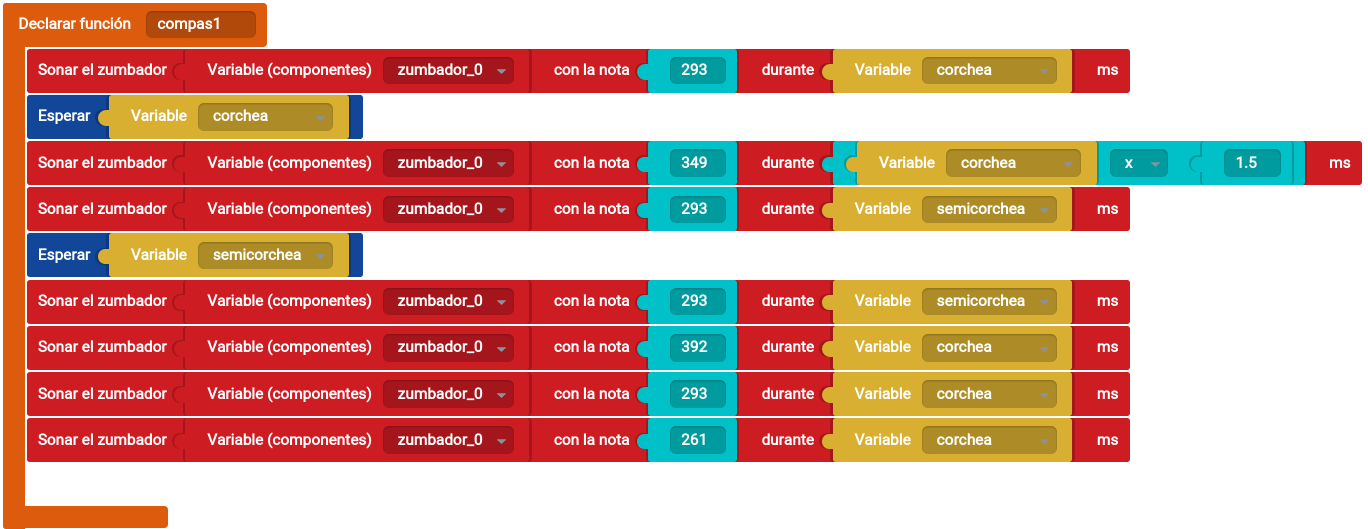
\includegraphics[width=12cm]{Figs/compas_bitbloq.png}
    \par
    \caption{\label{fig:bitbloq}Programando un ritmo musical mediantes bloques}
    \end{figure}

En el ámbito universitario, los dispositivos conectados permiten hoy en día acceder a un sinfín de información a través de Internet, ofreciendo a aquel que tenga interés en un tema la posibilidad de aprenderlo por sus propios medios. 
Las principales plataformas de robótica tienen disponibles sus propios tutoriales, donde destacan los de ROS o Robotic-Academy, aunque también se pueden encontrar en otras plataformas de cursos más generalistas. Otros recursos especializados son los disponibles en Robot Ignite Academy, pueden resultar de gran ayuda. 

\subsection{El entorno Robotics-Academy}
Dentro de la organización sin ánimo de lucro JdeRobot \cite{jderobot}, dedicada al desarrollo de software para robótica e Inteligencia Artificial, encontramos un conjunto de prácticas \textit{open-source} enfocadas al aprendizaje de distintos ámbitos relacionados con la robótica a través de código pyhton, compatibilidad con ROS y el uso del simulador Gazebo. Se trata de soluciones documentadas y en constante crecimiento, que han llegado a participar en el Google Summer of Code en tres ocasiones (2015,2017,2018).
Cada práctica enfrenta un problema típico diferente, dónde el estudiante encuentra una plantilla que le abstrae de toda la complejidad de bajo nivel del \textit{middleware} de manera que sólo deba preocuparse de sus algoritmos. 
Aunque se utiliza el simulador Gazebo para observar el comportamiento del robot con la solución, la adaptación para ejecutar las prácticas en robots reales es sencilla debido a que toda la configuración de la estructura y controladores del robot están definidos. A continuación se presentan algunas prácticas disponibles en Robotics-Academy:

El ejercicio de visión color filter, permite configurar un filtro  de color para realizar un filtrado sobre un objeto en las imágenes proporcionadas por un fichero de vídeo (ver Figura \ref{fig:colorFilter}). Por último, se debe detectar el movimiento de dicho objeto. Utiliza ICE como protocolo de comunicaciones y OpenCV para manejar las imágenes recibidas. 
Sobre tratamiento de imagen podemos encontrar también \textit{Follow Face}, que se encarga de detectar y perseguir caras en los fotogramas obtenidos por la cámara de vídeo \cite{Carlos}. 

\begin{figure}[hbt!]
\centering
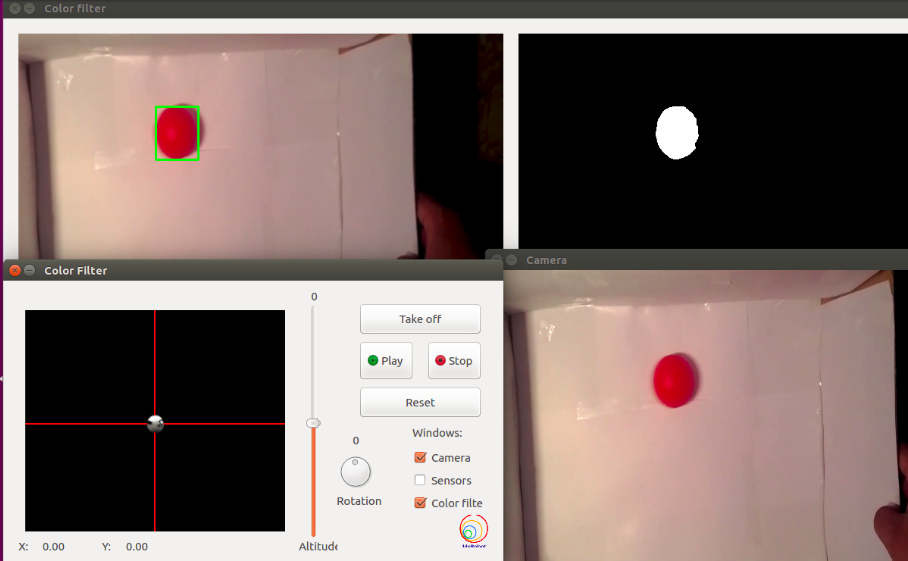
\includegraphics[width=12cm]{Figs/colorFilter.png}
\par
\caption{\label{fig:colorFilter}Filtro de color de la práctica color filter}
\end{figure}

En la práctica Drone cat\&mouse (ver Figura \ref{fig:catMouse}) dos drones deben jugar al gato y el ratón. Uno de ellos debe moverse de forma impredecible mientras el otro debe detectar el movimiento del otro y perseguirle, haciendo uso de las cámaras que lleva integradas y el procesamiento en tiempo real de las mismas. Este ejercicio fue utilizado en la competición \textit{program-a-robot}, celebrada en 2018 dentro del programa IROS(International Conference on Intelligent robots and Systems) y promovida por el grupo de robótica de la Universidad Rey Juan Carlos.

\begin{figure}[hbt!]
\centering
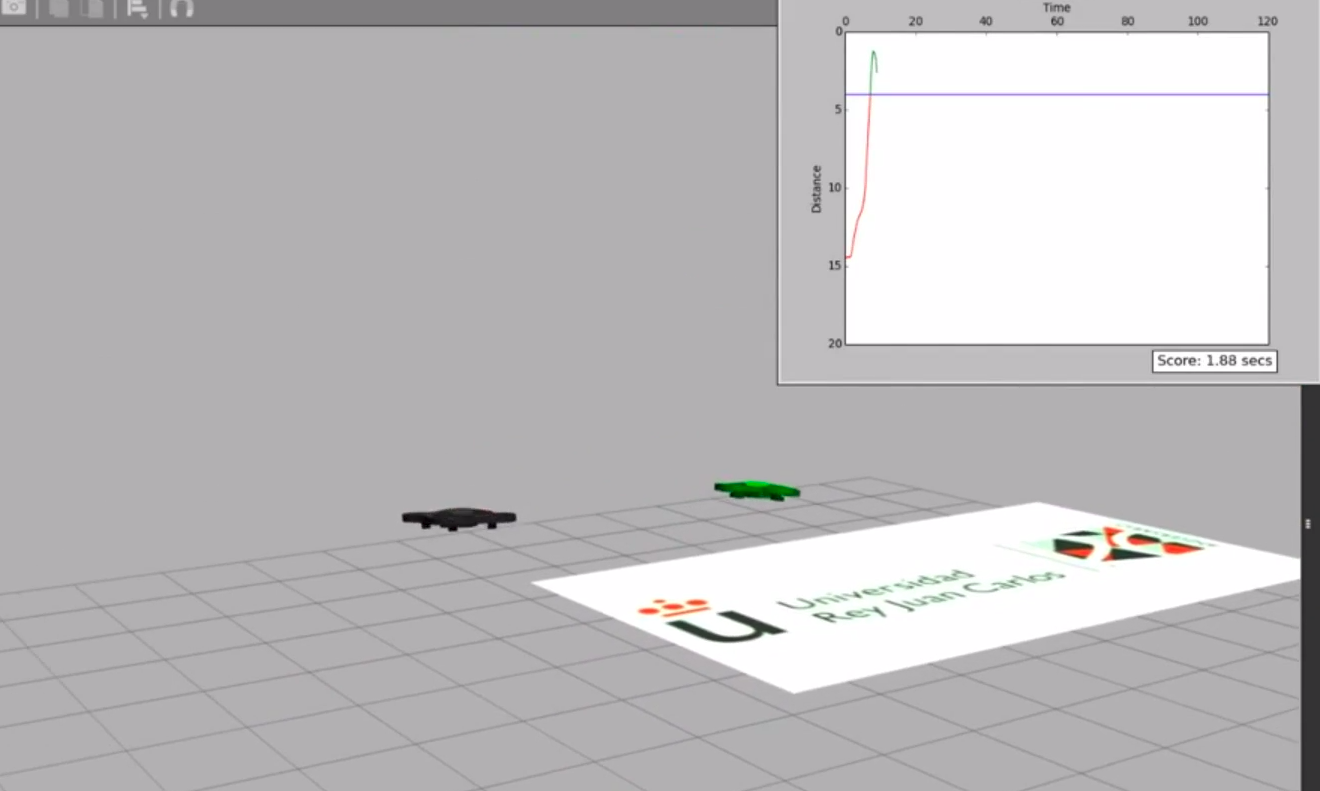
\includegraphics[width=12cm]{Figs/catMouse.png}
\par
\caption{\label{fig:catMouse}Persecución de drones en cat\&mouse}
\end{figure}

Entrando en el terreno de la autolocalización y aprovechando la potencia de los sensores de profundidad, la práctica Vacuum-cleaner with visualSLAM (ver Figura \ref{fig:vacuum}) permite simular el comportamiento de un robot aspirador de limpieza, detectando las partes de la casa por las que ha pasado y completando de forma eficiente el trabajo programado. En el mismo campo, la práctica Aspiradora autónoma \cite{Vanessa} permite familiarizarse con algoritmos de navegación. 

\begin{figure}[hbt!]
\centering
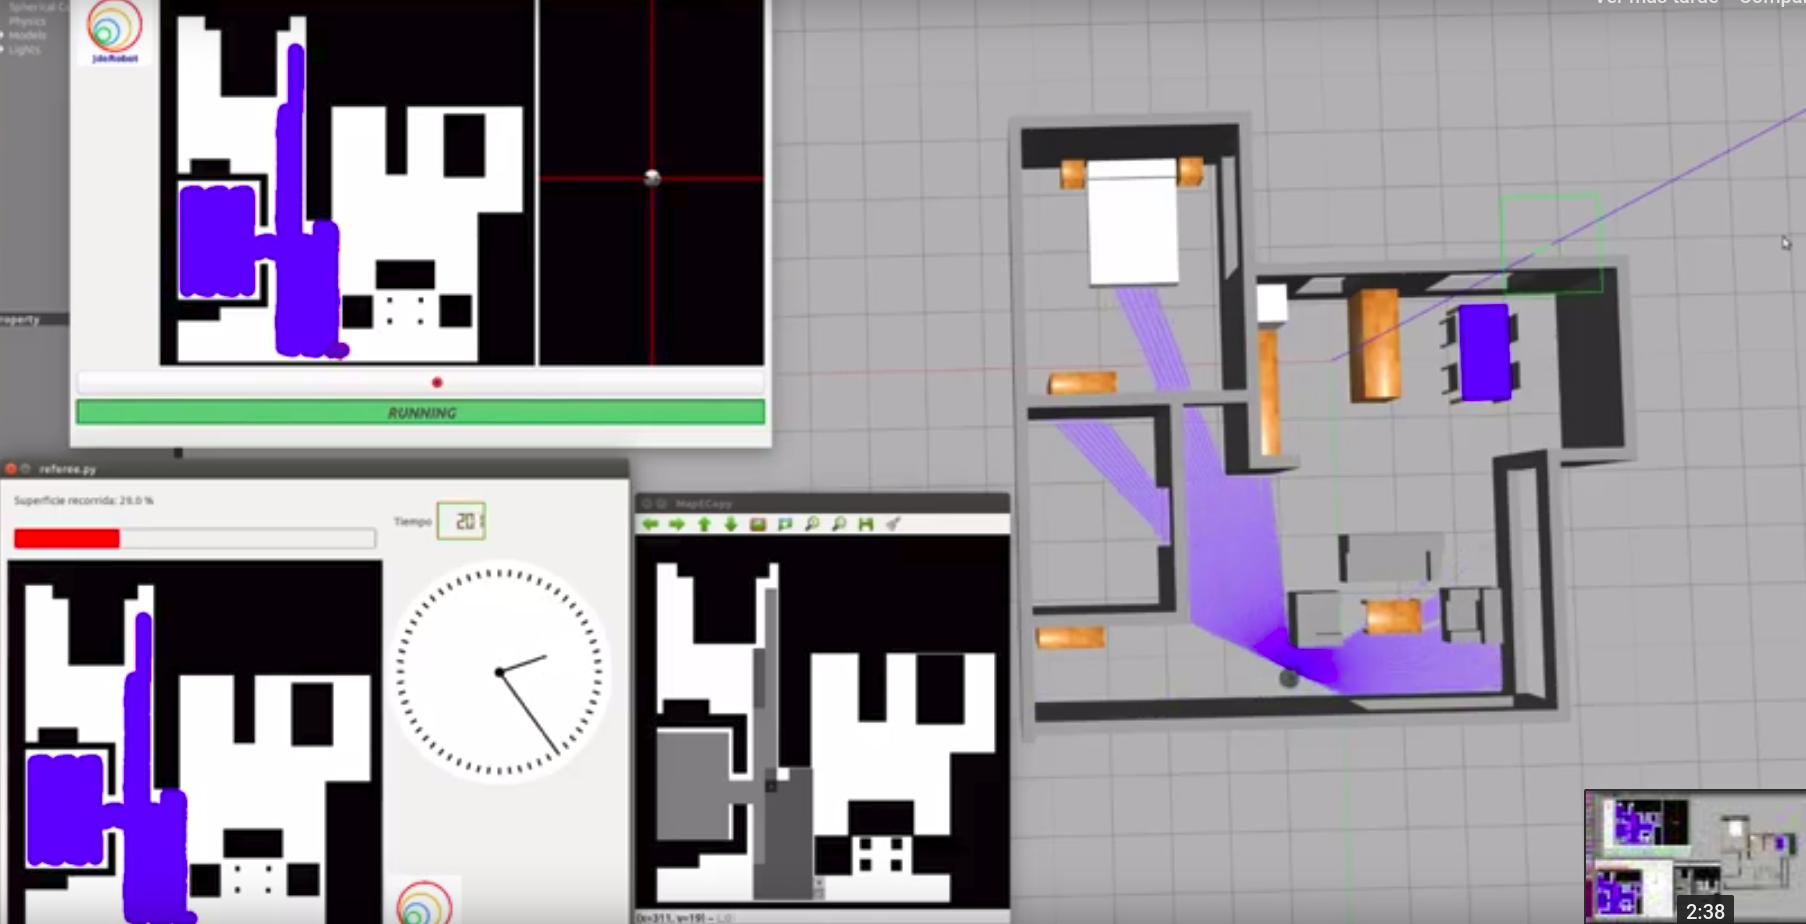
\includegraphics[width=12cm]{Figs/vacuumcleaner.png}
\par
\caption{\label{fig:vacuum}Mapeo generado en tiempo real en la práctica de la aspiradora}
\end{figure}

También hay ejemplos relacionados con los coches autónomos, como Visual follow-line behavior on a Formula1 (ver Figura \ref{fig:f1}) que permite a los estudiantes programar un Formula 1 que siga la línea roja en el centro de la carretera para dar una vuelta al circuito. Existen alternativas similares, que emplean drones en lugar de coches para seguir una determinada carretera \cite{Pablo}.

\begin{figure}[hbt!]
\centering
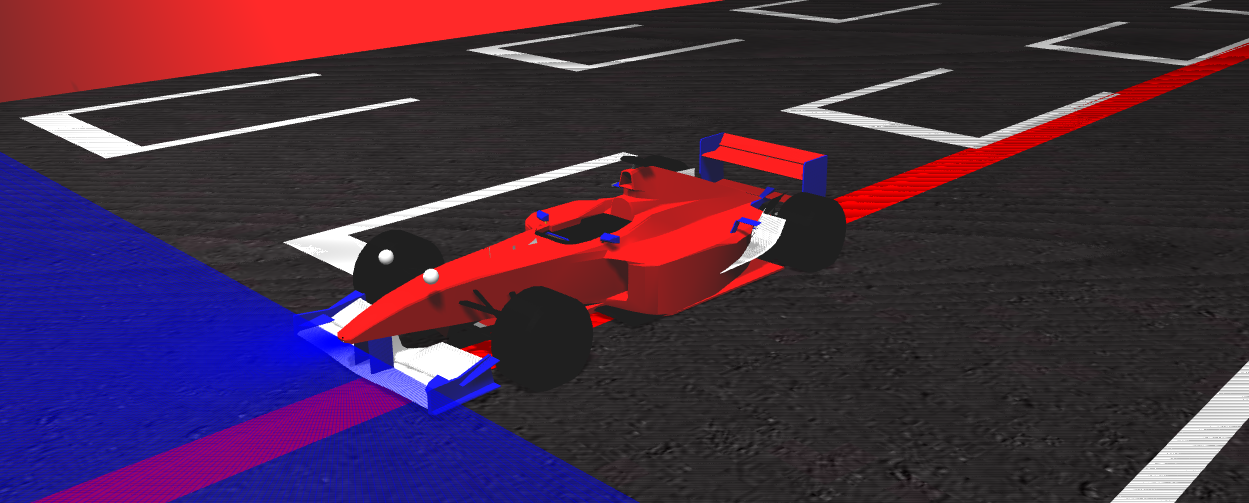
\includegraphics[width=12cm]{Figs/f1.png}
\par
\caption{\label{fig:f1}Mundo Gazebo para la práctica de conducción con Fórmula 1}
\end{figure}


\chapter{Objetivos}
Comprendido el contexto en que se ha desarrollado el proyecto, a continuación se
profundizará en los objetivos iniciales del mismo, los requisitos necesarios para el desarrollo de la solución, la metodología de trabajo y el plan de acción que se han seguido para alcanzarlos. 

\section{Objetivos}
El objetivo principal de este trabajo consiste en añadir una nueva práctica al entorno educativo Robotics-Academy de la organización JdeRobot. Dicha práctica tiene como meta profundizar en la planificación de trayectorias de un brazo robótico. Para realizar dicha práctica se utilizará MoveIt!, el entorno de ROS que ofrece herramientas para gestionar movimientos, manipulación, control, físicas y navegación. Además, se deben analizar y filtrar imágenes para detectar objetos y colores, para lo que será necesario conocer algunas de las posibilidades que ofrece la librería OpenCV. 

Para obtener la solución final, ha sido necesario plantear varios subobjetivos. El primero de ellos consiste en desarrollar la infraestructura necesaria, principalmente a través de un nuevo mundo generado en el simulador que incluirá los modelos para el robot y los distintos objetos. En segundo lugar se debe desarrollar una plantilla en Python que permita al receptor de la práctica tomar contacto con el tratamiento de imágenes y la planificación de trayectorias en MoveIt! de manera sencilla, abstrayéndole de los detalles de implementación más complejos, a los que podrá acceder posteriormente si desea profundizar en ellos. Por último, desarrollar la solución de referencia para lograr satisfacer el comportamiento esperado en esta práctica con un brazo robótico, incluyendo la planificación en entornos con obstáculos, la detección de objetos de color mediante procesado de imagen y la experimentación para optimizar los resultados. 

De esta forma el estudiante se podrá centrar en su desarrollo sin distraerse con problemas que ya han sido contemplados y resueltos, tomando contacto con la programación en robótica utilizando lenguaje Python y conociendo cómo funciona MoveIt!, a través de una práctica completa cuyo eje es la planificación.

\section{Requisitos}
A continuación, se enumeran las diferentes condiciones requeridas en el software y hardware para la consecución de los objetivos planteados: 
\begin{itemize}
    \item El software debe realizar acciones en tiempo real, con valores aceptables para los tiempos de ejecución en el simulador en un ordenador convencional.
    \item El software debe ser capaz de obtener trayectorias válidas en situaciones con varios obstáculos.
    \item Se utilizará el sistema operativo Ubuntu 16.04 LTS.
    \item El \textit{middleware} de referencia para trabajar es ROS en su versión Kinetic, debido a motivos de compatibilidad con su solución MoveIt!.
    \item El simulador de referencia es Gazebo 7, la versión recomendada para trabajar con ROS Kinetic. 
    \item El lenguaje de programación utilizado para los desarrollos es Python en su versión 2.7.12, nuevamente por razones de compatibilidad. Además, son necesarias nociones básicas de C++ para comprender el código de los repositorios de ROS. 
\end{itemize}

\section{Metodología}
La metodología de trabajo se ha basado en el modelo en espiral propuesto por primera vez en 1986 por el ingeniero Barry Boehm \cite{boehm}. Es un modelo iterativo, que enfoca los proyectos desde un punto de vista evolutivo, creciendo a partir de la realimentación y la definición periódica de objetivos. 
La propuesta original de Boehm se compone de las siguientes fases (ver Figura \ref{fig:spiralModel}), realizadas en bucle: 
\begin{itemize}
    \item Determinar objetivos. Incluye definir las tareas pendientes, las especificaciones, las restricciones y las estrategias para evitar riesgos.
    \item Análisis de riesgos. Consiste en estudiar las amenazas de cada etapa para tratar de minimizar los potenciales problemas y maximizar la eficiencia del trabajo. 
    \item Desarrollo y testing. En esta etapa, el ingeniero genera su solución, la verifica, y la valida. Es decir, se asegura de que se está desarrollando el producto como se ha definido y de que funciona como se espera que funcione. Parte de las tareas de pruebas consisten en anticipar errores, siendo éste uno de los principales ahorros de costes \cite{ibm_costs} \cite{inc_costs} que podemos encontrar en un proyecto software. 
    \item Planificación. Se revisa el estado de los objetivos y se definen las tareas a llevar a cabo con los recursos disponibles para la iteración en curso.  
\end{itemize}

\begin{figure}[hbt!]
\centering
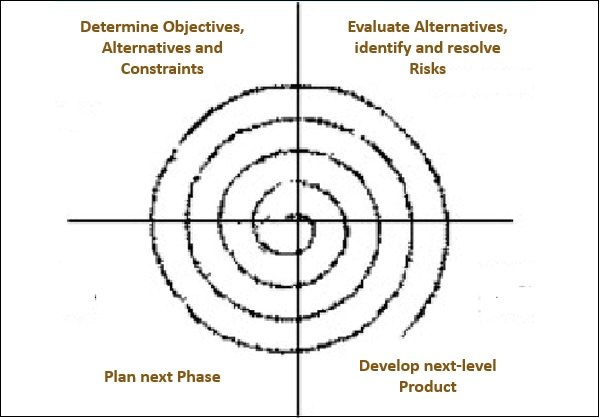
\includegraphics[width=12cm]{Figs/spiral_model.jpg}
\par
\caption{\label{fig:spiralModel}Representación gráfica del modelo en espiral para desarrollo software}
\end{figure}

Algunas de las ventajas de este modelo son la capacidad de adaptación, la reacción rápida frente a problemas, la reducción de riesgos y el enfoque realista. Sin embargo, también podría generar algunos inconvenientes, como la necesidad de un alto conocimiento de los posibles riesgos relativos al proyecto para no derivar en problemas en etapas avanzadas del desarrollo. 

La aplicación de los procedimientos propuestos por Boehm ha supuesto la realización de reuniones semanales de revisión del estado del proyecto, dónde se definen tareas, se proponen objetivos y se recopilan los avances. En la etapa de desarrollo, se ha ido alimentando una bitácora \cite{pages} con los hitos alcanzados y los problemas surgidos, además del repositorio disponible en GitHub \cite{repo}. Por tanto, se han gestionado los cambios con el sistema de control de versiones Git, añadiéndolos a la rama \textit{master} principal una vez validados.  

\section{Plan de acción}
Al enfrentar un proyecto de características técnicas, y marcar unos determinados objetivos, se debe marcar un plan de acción que determine cómo alcanzarlos, y de qué manera se lograrán. Para completar la práctica de planificación, se han requerido los siguientes pasos: 
\begin{itemize}
    \item Estudiar el lenguaje de programación C++ para poder comprender, y afrontar en caso de necesidad, los desarrollos necesarios para trabajar con robots.
    \item Familiarización con el entorno educativo Robotics-Academy a través de diversas prácticas para tomar contacto con la robótica y comenzar a comprender sus principios básicos. Este paso sienta las bases para poder comenzar a desarrollar el proyecto. 
    \item Conocer el simulador Gazebo a través de los tutoriales oficiales, y realizar la búsqueda de un robot comercial soportado completamente en el simulador. Incluye revisar los lenguaje de descripción URDF y SDF para construir mundos y modelos, y también cómo construir plugins para Gazebo. Posteriormente, utilizar dicho conocimiento para crear el mundo simulado para este ejercicio. 
    \item Descubrir y profundizar en el entorno de desarrollo software ROS, nuevamente a través de los tutoriales oficiales. Entre las acciones más importantes están construir espacios de trabajo, entender qué es un nodo ROS, como funciona ROS topics o aprender a generar ficheros \textit{roslaunch}.
    \item Comenzar a trabajar con MoveIt! a través de los tutoriales oficiales para ROS Kinetic, inicialmente para el robot PR2 y recientemente migrados a Panda. Algunas de las tareas clave han sido aprender a configurar robots, planificar y ejecutar movimientos, evitar obstáculos, añadir restricciones de planificación o utilizar correctamente el visualizador RVIZ. 
    \item Utilizar los conocimientos adquiridos para ofrecer una plantilla de código Python que abstraiga al usuario final de la complejidad de MoveIt! y OpenCV, y permita completar una práctica de planificación y ejecución de trayectorias con un brazo robótico en un entorno simulado. 
    \item Aplicar los conceptos previos para resolver los problemas necesarios y programar una solución de referencia para la práctica de robótica escogida.
    
\end{itemize}

\chapter{Infraestructura utilizada}
En este capítulo se detalla el software que se ha empleado para el desarrollo del TFG. Desde ROS Kinetic y JdeRobot como \textit{middleware}s robóticos, pasando por la herramienta MoveIt! para facilitar el trabajo con robots hasta llegar al simulador Gazebo. Todo ello corriendo en el sistema operativo Ubuntu 16.04 y desarrollado en Python.  Las comunicaciones entre los distintos componentes utilizan principalmente ROS topics. 

\section{Robot PR2}
El robot (ver Figura \ref{fig:pr2}) sobre el que se ha desarrollado el software es el modelo PR2 \cite{pr2} de la empresa Willow Garage, especializada en robótica y responsable en su día también del software ROS y otras herramientas de código abierto. El nombre viene de Personal Robot 2, haciendo referencia a la idea de que fuera un asistente en casa y no un robot industrial como la mayoría de los comercializados hasta el momento de su lanzamiento. 

\begin{figure}[hbt!]
\centering
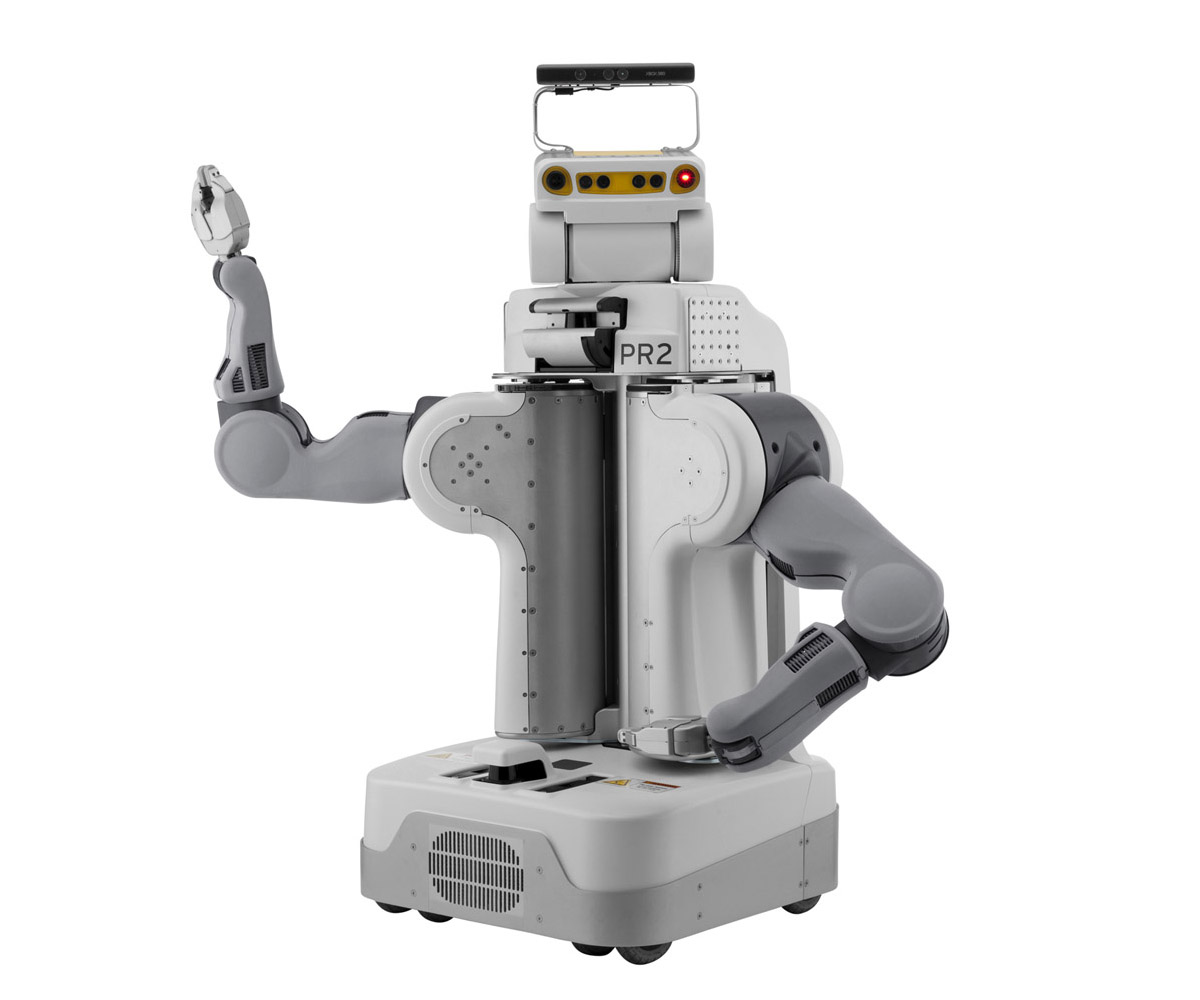
\includegraphics[width=12cm]{Figs/PR2_image.jpg}
\par
\caption{\label{fig:pr2}Imagen de un robot PR2 real}
\end{figure}

Se compone de dos brazos (derecho e izquierdo) capaces de generar un amplio abanico de oportunidades de movimiento que no serían posibles con un único brazo, y que terminan en una pinza o \textit{gripper} que permite agarrar objetos.
Su diseño modular (ver Figura \ref{fig:pr2Structure}) permite integrarlo con otros \textit{grippers}, brazos o sensores.

\begin{figure}[hbt!]
\centering
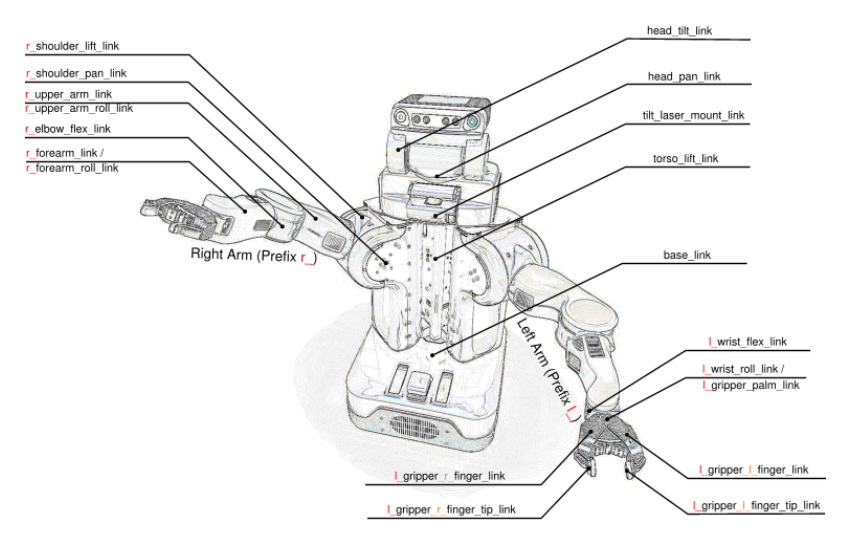
\includegraphics[width=12cm]{Figs/PR2_structure.png}
\par
\caption{\label{fig:pr2Structure}Estructura del robot PR2}
\end{figure}

Su muñeca tiene dos grados de movimiento, que se suman a la libertad que aportan las articulaciones del hombro y el codo para permitir prácticamente cualquier movimiento necesario para una labor doméstica.

Además de su estructura, una característica fundamental del robot PR2 son las cámaras y láseres que permiten conocer el entorno y actuar según lo que percibe: detectar objetos, saber a qué distancia se encuentran e identificar zonas objetivo permiten llevar a cabo acciones como abrir una puerta o llevar objetos de un lugar a otro.

\subsection{Cámara Microsoft Kinect}
La cámara Kinect (ver Figura \ref{fig:kinect}), que ha sido incorporada al PR2 canónico para poder obtener imágenes desde la perspectiva del robot, permite conocer el entorno a través de imágenes procesadas en tiempo real. 
Contiene un sensor de color RGB y uno de profundidad, y se sitúa en la parte superior del robot. 

Kinect es propiedad de Microsoft, y fue lanzada originalmente en el año 2010 con el objetivo de ofrecer nuevas posibilidades para su consola Xbox, aunque fue perdiendo protagonismo con el paso de los años. Más tarde se comercializó también para ordenadores, dando el salto así a proyectos de índole científica que se sirven de su detección de movimiento y reconocimiento de voz. 

\begin{figure}[hbt!]
\centering
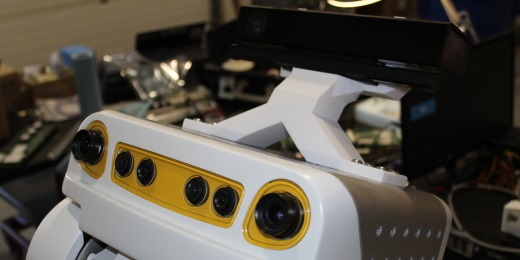
\includegraphics[width=12cm]{Figs/kinect.jpg}
\par
\caption{\label{fig:kinect}Apariencia de una cámara Kinect de Microsoft}
\end{figure}

\section{Simulador Gazebo}
Este simulador \textit{open source} nació en el año 2002 en la Universidad del Sur de California (USC) como proyecto entre un profesor y uno de sus estudiantes. El objetivo era poder trabajar con robots bajo condiciones de alta fidelidad, pensando principalmente en entornos exteriores. Se comenzó a integrar con ROS en 2009 y dos años después la citada Willow Garage comenzó a financiar el desarrollo para este software, del que se hizo cargo la Open Source Robotics Foundation (OSRF).
Gazebo \cite{gazebo} fue adaptado para participar en la prestigiosa DARPA Robotics Challenge (DRC) en el año 2013. Hay una comunidad activa detrás del proyecto que permite introducir mejoras, resolver bugs y consultar dudas técnicas.

Como simulador de robótica de referencia para esta práctica y los desarrollos sobre ROS en general, permite crear aplicaciones para robots sin necesidad de depender de la máquina física. Así, las aplicaciones creadas para un modelo concreto podrán utilizarse posteriormente en el mundo real sin  realizar muchas modificaciones, disminuyendo tanto los costes económicos como los derivados de las pruebas en fase de desarrollo que pueden dañar el robot. 
Ofrece visualización 3D y un potente motor de físicas (ver Figura \ref{fig:gazeboExample}) para, en el caso de un brazo robótico, poder determinar parámetros como fricción, rango de movimiento o colisiones.

\begin{figure}[hbt!]
\centering
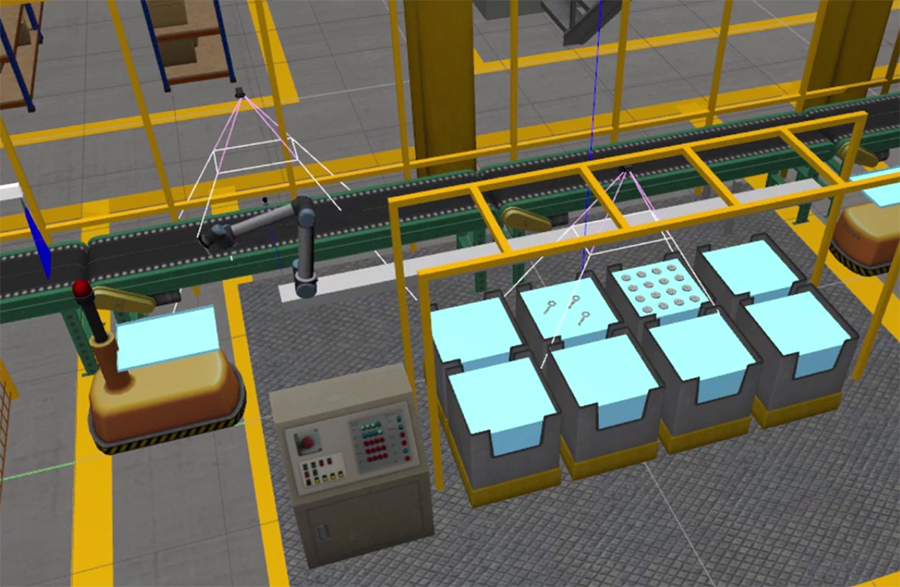
\includegraphics[width=12cm]{Figs/gazebo_example.jpg}
\par
\caption{\label{fig:gazeboExample}Mundo Gazebo que simula un entorno industrial}
\end{figure}

La simulación nace a partir de un fichero \textit{.launch} que arranca Gazebo. El entorno de la simulación está compuesto por un mundo que contiene diferentes modelos. Estos modelos están definidos en un fichero con formato SDF con los siguientes componentes principales:

\begin{itemize}
\item \textit{Links}: contiene las propiedades físicas de un trozo del modelo, incluyendo algunas de visualización y colisión, sensores, inercias o iluminación.
\item \textit{Joints}: conexión entre dos links.
\item \textit{Plugins}: librería externa que controla un modelo. 
\end{itemize}

La versión utilizada para este proyecto es Gazebo7.

\section{Middleware robótico ROS Kinetic}
ROS es un entorno para el desarrollo de software para robots. Nació en 2007 en el Laboratorio de Inteligencia Artificial de Standford. La arquitectura de grafos de ROS (Robot Operating System) se basa en nodos que se comunican a través de mensajes. La práctica con un brazo robótico desarrollada tendrá como eje un nodo ROS que se comunicará con los drivers del PR2 en Gazebo y con las librerías de manejo de imágenes y planificación. 

Es un sistema de código abierto que encarga de mantener la OSRF (Open Source Robotics Foundation). Aporta al usuario herramientas como por ejemplo planificación de movimiento (MoveIt) o reconocimiento del entorno y visualización (RVIZ), además de soporte para un amplio abanico de Robots. 

La versión Kinetic fue lanzada en mayo de 2016, enfocada al uso desde Ubuntu 16.04. La versión Gazebo7 es la recomendada en ROS Kinetic para este simulador. 

Un paquete de ROS agrupa varios programas o nodos con funcionalidades similares. Estos nodos se comunican  a través de mensajes, llamados \textit{ROS Topics}, que les permiten interactuar entre sí, y pueden estar programados en distintos lenguajes como Python y C++.
ROS Core es la herramienta encargada de arrancar el nodo máster y gestionar todas las comunicaciones, por lo que es la primera que debe ser arrancada. 

Un nodo ROS se puede lanzar automáticamente a través de  ficheros \textit{.launch}, que serán muy habituales en el desarrollo. 

Para ejecutar un nodo, necesitaremos el paquete y el nombre del nodo. Una vez lanzado el nodo, podemos publicar \textit{topics} de un tipo concreto que el nodo comprenda, consiguiendo así que realice una acción determinada. Podemos consultar en cualquier momento la lista de los nodos o \textit{topics} disponibles, o ver los mensajes publicados en un determinado \textit{topic}. (ver Algoritmo \ref{alg:roscommands}).

\begin{algorithm}[htb!]
	\begin{lstlisting}[breaklines=true,language=python]
# Para lanzar un nodo turtlesim y publicar un mensaje en el topic /turtle1/cmd_vel
$ roscore
$ rosrun turtlesim turtlesim_node
$ rostopic pub -1 /turtle1/cmd_vel geometry_msgs/Twist -- '[2.0, 0.0, 0.0]' '[0.0, 0.0, 1.8]'
# Para obtener los mensajes publicados en el topic: 
$ rostopic echo /turtle1/cmd\_vel
# Para representar gráficamente las comunicaciones actuales:
$ rosrun rqt_graph rqt_graph
# Para obtener los nodos y topics disponibles: 
$ rosnode list 
$ rostopic list
	\end{lstlisting}
\caption{\label{alg:roscommands}Comandos básicos para trabajar con ROS desde un terminal Linux}
\end{algorithm}

Las comunicaciones entre nodos son la base del desarrollo con robots en ROS, y son representables en forma de grafo a través de la herramienta \textit{rqt} (ver Figura \ref{fig:turtlesim}).

\begin{figure}[hbt!]
\centering
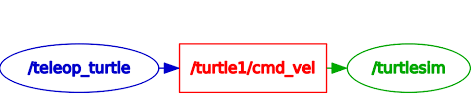
\includegraphics[width=12cm]{Figs/turtle_graph.png}
\par
\caption{\label{fig:turtlesim}Representación gráfica utilizando \textit{rqt} de un nodo teleoperador comunicándose con un nodo tortuga a través de un \textit{topic}}
\end{figure}

\section{Lenguaje de programación C++}
Este lenguaje de programación fue creado por Bjarne Stroustrup en 1979, que lo bautizó en sus inicios como ‘C con clases’. No en vano tiene una sintaxis similar a la de C, manteniendo el vínculo con el lenguaje del que proviene y añadiendo mecanismos de programación orientada a objetos a su predecesor. Su nombre además hace referencia a ese C incrementado, mejorado. 
Es un lenguaje fuertemente tipado y portátil. Se rige por un estándar de ISO (International Organization for Standardization) cuya última versión es C++17, lanzada en 2017. 

Es lenguaje con un grado de complejidad elevado, que permite una gran versatilidad y potencia, pero también tiene una curva de aprendizaje elevada para dominarlo.
Algunos IDEs recomendados para trabajar con C++ son VisualStudio y Code::Blocks. 
Como curiosidad, se trata del cuarto lenguaje de programación más popular hoy en día según el conocido ranking de TIOBE \cite{tiobe}, sólo por detrás de Java, C y Python. Alcanzó su máximo de popularidad 2003 según los datos de esta empresa de software. 

\section{Lenguaje de programación Python}
Fue creado en los años 80 por Guido van Rossum. Es un lenguaje de programación interpretado, que utiliza tipado dinámico. Su sintaxis está enfocada a ser fácilmente legible, lo que hace que tenga una curva de aprendizaje suave en relación con otros lenguajes como Java o el propio C. Soporta programación orientada a objetos y es multiplataforma.

Una característica interesante es que puede extenderse con módulos de C o C++.
Según el mencionado ranking TIOBE, Python es el tercer lenguaje de programación en popularidad, alcanzando en 2019 su máximo nivel en la lista. 

Se ha utilizado la versión 2.7.12 debido principalmente a su compatibilidad con ROS Kinetic. En este lenguaje se han desarrollado la plantilla y la solución de referencia para la aplicación de planificación de movimientos 

\section{Biblioteca de visión OpenCV}
Es una biblioteca de código abierto enfocada a proyectos de visión artificial, con interfaces disponibles para varios lenguajes de programación (C++, Python, Java, MATLAB...). Open Source Computer Vision Library (OpenCV) \cite{opencv} es muy utilizada, con un número de descargas de alrededor de 15 millones y una comunidad de 47000 seguidores. Este dato está potenciado por el hecho de ser multiplataforma, soportando sistemas Windows, Linux, MacOS, Android e iOS. 
Algunos ejemplos de uso de la librería son compañías de la envergadura e influencia de Google, Yahoo, Microsoft, Intel, IBM, Sony, Honda o Toyota.

Los algoritmos que contiene están desarrollados de forma nativa en C++ debido a su mayor rendimiento en comparación con los demás lenguajes. El resto de ellos utilizan interfaces para acceder a toda la funcionalidad disponible. 
En el caso de Python, se utiliza a través del paquete cv2, que internamente utiliza la librería Numpy, altamente optimizada e indicada para el cálculo científico y las operaciones matemáticas con matrices. 

Su integración en el proyecto permite aprovechar toda la potencia del análisis de imágenes en un entorno robótico para, en este caso, analizar imágenes de lo que observa el robot y poder detectar objetos de color dinámicamente. En este trabajo se ha empleado la versión 3.3.1.

\section{Entorno de planificación de movimientos MoveIt!}
MoveIt! nació en octubre del año 2011 con la idea de agrupar todos los avances relacionados con planificación de movimientos, manipulación, percepción 3D, cinemática, control y navegación en una única herramienta. Actualmente es el software de código abierto más utilizado para manipulación con robots, con más de 65 autómatas soportados. 

Tiene un nodo principal llamado \textit{move\_group } que actúa como integrador, permitiendo a todos los componentes comunicarse entre sí realizando las acciones soportadas. 
Se puede acceder a \textit{move\_group } por tres vías: C++, Python y RVIZ.
\begin{figure}[hbt!]
\centering
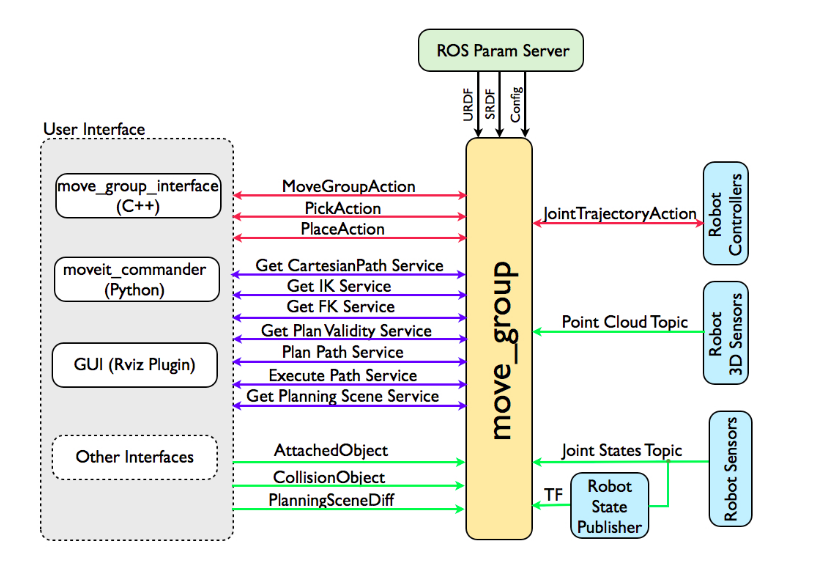
\includegraphics[width=12cm]{Figs/moveGroup.png}
\par
\caption{\label{fig:moveGroup}Resumen esquematizado de las posibles interacciones que ofrece \textit{move\_group}}
\end{figure}
El nodo \textit{move\_group} necesita varios parámetros de entrada (ver Figura \ref{fig:moveGroup}):
\begin{itemize}
\item URDF (Universal Robot Description Format): Es el formato que utiliza ROS para la descripción del robot. Se ha utilizado el del paquete \textit{pr2\_description}, correspondiente al autómata utilizado.
\item SRDF (Semantic Robot Description Format) complementa al URDF, añadiendo más información como grupos de joints, configuraciones por defecto para el robot o chequeo de colisiones. Para construir este fichero, se recomienda utilizar el MoveIt! Setup Assistant. Esta herramienta permite configurar cualquier robot para ser utilizado en MoveIt! A través de una interfaz gráfica que simplifica el trabajo. 
\item MoveIt! Configuration: Incluye otros ficheros de configuración específicos de MoveIt!, normalmente generados también a través del Setup Assistant. Contienen información necesaria para planificación de movimientos, cinemática o percepción del entorno.
\end{itemize}
Las principales interfaces de MoveIt! permiten acceder a las diferentes funcionalidades a través de código C++. Sin embargo, existe un paquete llamado \textit{moveit\_python} que permite acceder a las principales interfaces de MoveIt! utilizando Python:
\begin{itemize}
\item MoveGroupInterface: Utilizada para acceder a \textit{move\_group } y mover el brazo. 
\item PlanningSceneInterface: Utilizada para añadir o eliminar objetos al entorno y cambiar su apariencia, ya sean conectados o de colisión. 
\end{itemize}

Con el objetivo de conseguir la integración de MoveIt! con Gazebo, y poder así enviar los movimientos al robot real o simulado, debemos configurar correctamente los controladores. Para ello necesitaremos dos ficheros clave: \textit{controllers.yaml} y \textit{joint\_names.yaml}.  En ellos se especifican el tipo de mensajes que el robot recibe y las articulaciones que controla.  

Al tratarse de la principal herramienta utilizada para completar el ejercicio, su funcionamiento y la manera en la que se ha empleado se detallarán en los siguientes capítulos.

\chapter{Ejercicio de planificación de trayectorias con brazo robótico}
En este capítulo se describirán en detalle tanto el objetivo como el desarrollo técnico de la práctica "Movimiento planificado de un brazo robótico" \ para el entorno Robotics-Academy. 
El capítulo incluye el enunciado de la práctica, la infraestructura específica necesaria y la plantilla de código Python desarrollada para albergar la solución del estudiante. 

\section{Enunciado}
 El objetivo de este ejercicio consiste en un robot PR2 que debe observar un objeto y planificar un movimiento con el brazo izquierdo sorteando obstáculos, hasta golpear un objeto final que será del mismo color que el observado al comienzo. Incluye por tanto la planificación de trayectorias con obstáculos en un entorno simulado, el reconocimiento de objetos analizando espacios de color, y la ejecución de movimientos. Se utilizarán la librería OpenCV para el análisis de imágenes y el paquete MoveIt! para la fase de planificación. 

\begin{figure}[hbt!]
\centering
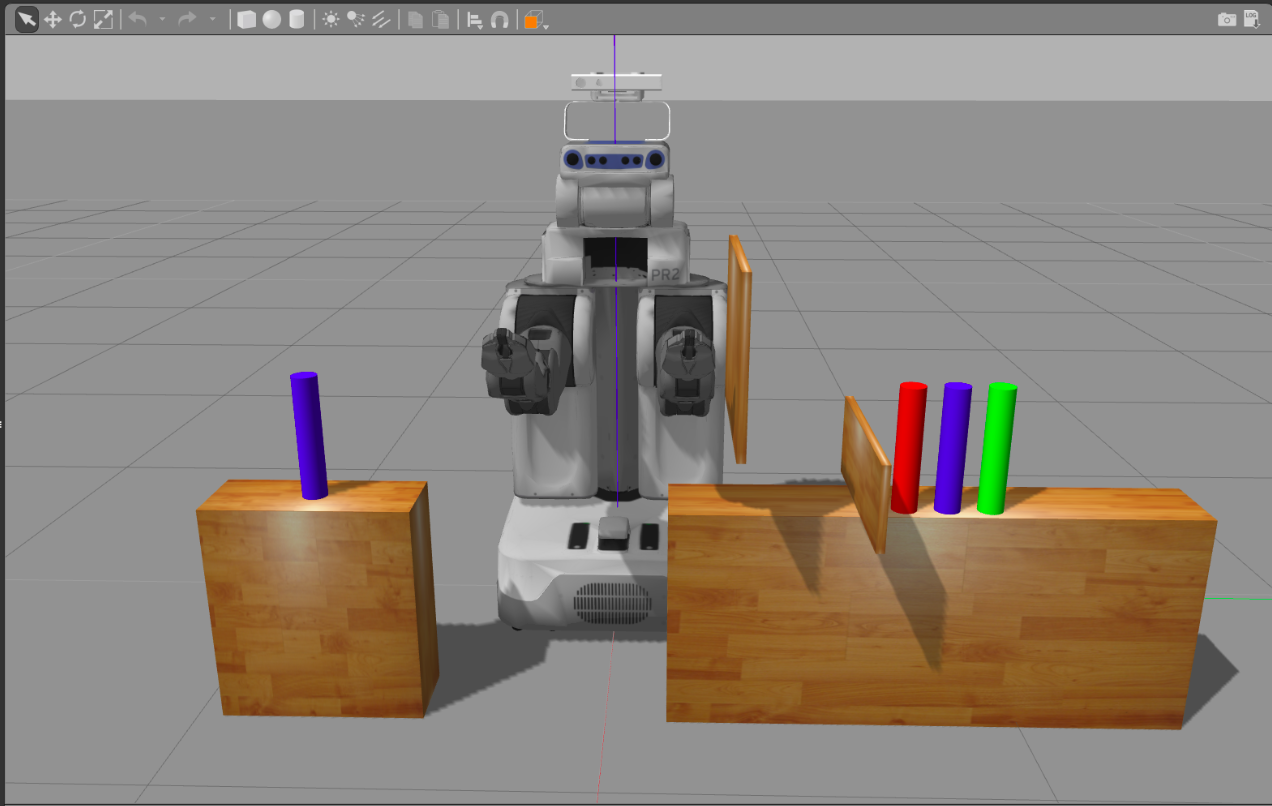
\includegraphics[width=12cm]{Figs/tfg_gazebo_world.png}
\par
\caption{\label{fig:Mundo-gazebo}Mundo Gazebo que incluye todo lo necesario para el desarrollo de la práctica: zonas, objetos, robot y obstáculos.}
\end{figure}

El escenario de la práctica contiene un mundo Gazebo (ver Figura \ref{fig:Mundo-gazebo}) que incluye dos zonas de acción (muestra y derribo) y un total de cuatro objetos, uno en la primera zona y tres en la segunda. Entre ellas, un robot PR2 y algunos obstáculos. Los objetos en la zona de derribo tendrán los colores rojo, verde y azul, y el de la zona de muestra tiene únicamente uno de los colores mencionados (azul por defecto). 

La ejecución típica comienza con el robot PR2 moviendo la cabeza y observando la zona de muestra. En ese momento, debe ser capaz de obtener las imágenes de la cámara Kinect que incorpora, que serán analizadas mediante código Python para determinar si hay o no un objeto y de qué color es. 
Después, conociendo el color objetivo y las posiciones de los objetos en la zona de derribo, será capaz de planificar, y posteriormente ejecutar, una trayectoria con su brazo izquierdo que le sitúe frente al objeto en la zona de derribo cuyo color coincida con el observado en la zona de muestra. Para ello será necesario gestionar la planificación de trayectorias evitando los obstáculos necesarios para, por último, realizar un movimiento de derribo.

\section{Diseño}
La estructura diseñada (ver Figura \ref{fig:tfg_schema}) tiene como núcleo el sistema ROS. A través de él, el nodo creado puede comunicarse con el simulador y las librerías externas. La interacción con el simulador debe ser bidireccional ya que ambos deben conocer qué está ocurriendo al otro lado; el modelo del robot en Gazebo necesita recibir mensajes para saber hacia dónde moverse, así como la planificación de trayectorias dirigida por MoveIt! necesita saber la posición actual para enviar sus mensajes de movimiento.

\begin{figure}[hbt!]
\centering
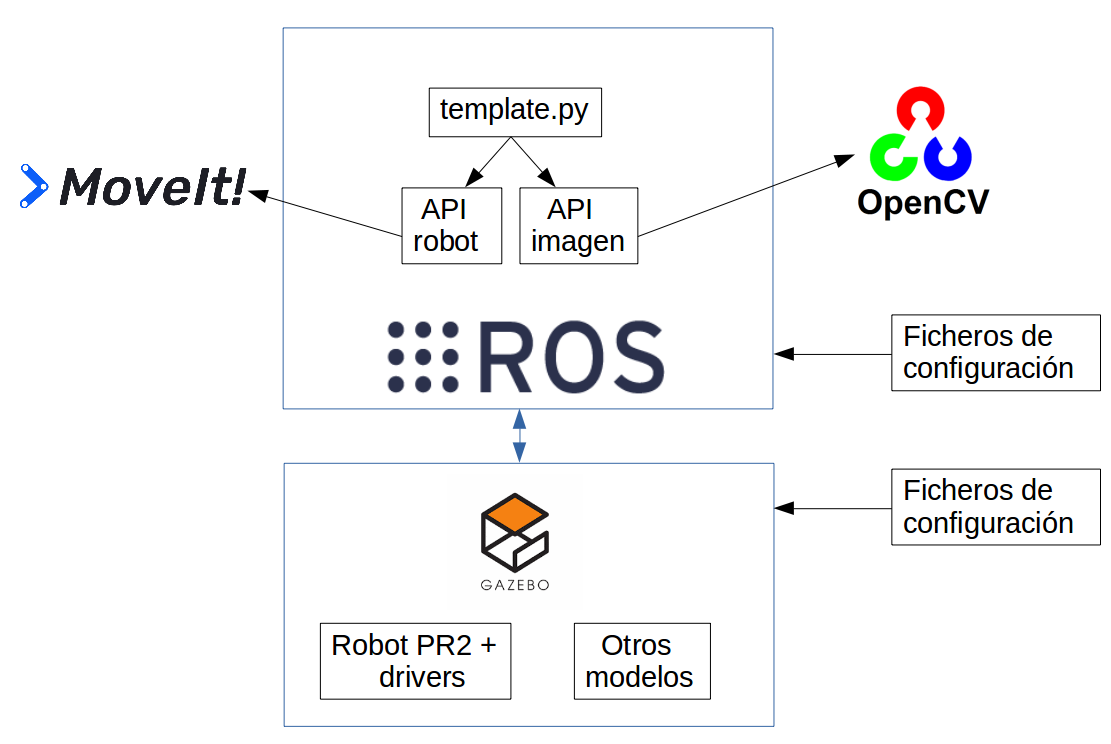
\includegraphics[width=12cm]{Figs/tfg_schema.png}
\par
\caption{\label{fig:tfg_schema}Esquema de la arquitectura software utilizada.}
\end{figure}

Por su parte, el simulador Gazebo contiene el modelo del robot, incluyendo sus controladores, así como el resto de modelos necesarios, como las zonas de acción, los objetos y los obstáculos.  

El nodo ROS principal, ofrece las APIs de manejo de imágenes y de manejo del robot, que son utilizadas desde la plantilla codificada en Python. Para ofrecer las funcionalidades disponibles a través de dichas interfaces de programación, son necesarias las librerías OpenCV y MoveIt!.

\section{Infraestructura del ejercicio}\label{sec:infraestructura}
Los elementos necesarios para lograr esta práctica completa de planificación son el mundo creado en Gazebo y todos los objetos estáticos que contiene (mesas, obstáculos, cilindros de colores), el robot PR2 y sus drivers para las articulaciones y la captura de imágenes, y los plugins utilizados para la captura de imagen.  

\subsection{Mundo Gazebo}
En primer lugar, ha sido necesaria la creación de un mundo en Gazebo (ver Figura \ref{fig:Mundo-gazebo}) que contiene los objetos a detectar y empujar, las dos zonas de acción, los obstáculos, el robot PR2 y la cámara Kinect.

La cámara Kinect se incorpora en la parte superior de la cabeza del robot, de forma que se encuentran completamente integrados y podemos controlar la visión del robot a través de movimientos en su parte superior.
Utiliza el plugin openni\_Kinect (ver Algoritmo \ref{alg:kinect2-xacro}), que permite obtener imágenes con resolución 680x480 y formato BGR, con 8 bits para cada uno de los colores primarios de la luz y por tanto un total de 24 bits por píxel. Además, al tratarse de una de las comúnmente llamadas cámara RGB-D, ofrece imágenes de profundidad que permitirían detectar lo cerca o lejos que se encuentra un objeto de la cámara. 

\begin{algorithm}[htb!]
	\begin{lstlisting}[breaklines=true,language=python]    
<xacro:macro name="kinect2_rgb_gazebo_v0" params="link_name frame_name camera_name">
  <gazebo reference="${link_name}">
    <sensor type="depth" name="${name}_rgb_sensor">
      <always_on>true</always_on>
      <update_rate>1.0</update_rate>
      <camera>
        <horizontal_fov>${57.0*M_PI/180.0}</horizontal_fov>
        <image>
          <format>B8G8R8</format>
          <width>640</width>
          <height>480</height>
        </image>
        <clip>
          <near>0.01</near>
          <far>5</far>
        </clip>
      </camera>
      <plugin name="${link_name}_controller" filename="libgazebo_ros_openni_kinect.so">
        <alwaysOn>true</alwaysOn>
        <updateRate>1.0</updateRate>
        <cameraName>${camera_name}_rgb</cameraName>
        <imageTopicName>/${camera_name}/rgb/image_raw</imageTopicName>
        <cameraInfoTopicName>/${camera_name}/rgb/camera_info</cameraInfoTopicName>
        <depthImageTopicName>/${camera_name}/depth/image_raw</depthImageTopicName>
        <depthImageCameraInfoTopicName>/${camera_name}/depth/camera_info</depthImageCameraInfoTopicName>
        <pointCloudTopicName>/${camera_name}/depth_registered/points</pointCloudTopicName>
        <frameName>${frame_name}</frameName>
        <pointCloudCutoff>0.5</pointCloudCutoff>
      </plugin>
    </sensor>
    <material value="Gazebo/Red" />
  </gazebo>
</xacro:macro>
	\end{lstlisting}
\caption{\label{alg:kinect2-xacro}Extracto del fichero kinect2.gazebo.xacro, donde se define el plugin para la cámara}
\end{algorithm}

Para lanzar este entorno, se debe ejecutar un fichero \textit{.launch} (ver Algoritmo \ref{alg:tfg-launch}), que pondrá en funcionamiento los modelos necesarios para las dos zonas de referencia, los modelos de los objetos y obstáculos, y el robot PR2 con todos sus controladores. La cámara Kinect integrada se pasa como parámetro, aunque está configurada para aparecer por defecto. Se puede lanzar el mundo escribiendo en un terminal siguiente comando:

\$\ \ \ \ roslaunch pr2\_gazebo tfg\_launch.launch

\begin{algorithm}[htb!]
\begin{lstlisting}[breaklines=true,language=python]
<launch>
  <!-- start up world -->
  <arg name="gui" default="true"/>
  <arg name="headless" default="false" />
  <arg name="debug" default="false" />
  <arg name="paused" default="true"/>
  <arg name="KINECT2" default="$(optenv KINECT2 true)" />
  <include file="$(find gazebo_ros)/launch/empty_world.launch">
    <arg name="world_name" value="worlds/tfg_world.world"/> 
    <arg name="gui" value="$(arg gui)" />
    <arg name="headless" value="$(arg headless)" />
    <arg name="paused" value="$(arg paused)" />
    <arg name="debug" value="$(arg debug)" />
    <arg name="use_sim_time" value="true" />
  </include>
  <!-- start pr2 robot with Kinect camera -->
  <include file="$(find pr2_gazebo)/launch/pr2.launch">
    <arg name="KINECT2" value="$(arg KINECT2)" />
  </include>
</launch>
\end{lstlisting}

\caption{\label{alg:tfg-launch}Fichero \textit{.launch} para el mundo gazebo y el robot PR2.}
\end{algorithm}

\subsubsection{Modelo PR2 enriquecido}
El modelado principal del robot PR2 utilizado en esta práctica corresponde a los paquetes \textit{pr2\_gazebo} y \textit{pr2\_common}. Se trata de paquetes disponibles para ROS Kinetic, que contienen todo lo necesario para simular el robot de Willow Garage en Gazebo, como  información sobre articulaciones, físicas, colisiones o dimensiones. 

De cara a lograr el objetivo final, ha sido necesario hacer ligeras modificaciones. En primer lugar, para añadir una cámara Kinect \cite{gazebo_plugins} en la parte alta del modelo. Esta es una opción disponible en el paquete original pero que debemos configurar como opción por defecto (la original lanza el robot sin ninguna cámara), utilizando el argumento KINECT2 al lanzar el fichero \textit{.launch} del robot PR2. 

En segundo lugar, en la fase inicial de pruebas con reconocimiento de imagen en el entorno creado, se evidenciaban problemas a la hora de detectar los colores a causa del sensor láser incluido por defecto en el modelo. El sensor generaba ruido en las imágenes RGB obtenidas, dificultando la caracterización de los objetos, motivo que provocó su desactivación en los paquetes generados.    

Para llevar a cabo estas modificaciones, es necesario conocer el concepto de \textit{overlaying} \cite{overlaying}, utilizado en ROS para hablar de modificaciones en el espacio de trabajo \cite{wstool} del usuario sobre los paquetes originales descargados de los repositorios oficiales. De esta manera podemos hacer que ROS priorice nuestros propios repositorios, donde se habrán modificado los ficheros necesarios para lograr un determinado funcionamiento, como por ejemplo la desactivación del sensor láser.

\subsubsection{Modelos adicionales}
Se ha desarrollado un fichero .world (ver Algoritmo \ref{alg:model}) que define los modelos necesarios para la consecución de la práctica. Para cada uno de los elementos se establecen su posición, cómo será su visualización, sus criterios de colisión y sus dinámicas. 
Para ello se utiliza el formato SDF \cite{sdf_format}, de código abierto y basado en XML, que permite describir modelos de cualquier complejidad a través de sencillas etiquetas, desde esferas o prismas, hasta robots completos.

\vspace{20pt}
\begin{algorithm}[htb!]
	\begin{lstlisting}[breaklines=true,language=python]  
  <model name="base_A">
   <pose>0.6 -0.7 0.275 0 0 0</pose>
   <static>true</static>
   <link name="link">
    <collision name="surface">
     <pose>0.0 0.0 0.0 0 0 0</pose>
     <geometry>
      <box>
       <size>0.2 0.5 0.55</size>
      </box>
     </geometry>
     <surface>
      <friction>
       <ode>
        <mu>10</mu>
        <mu2>10</mu2>
       </ode>
      </friction>
     </surface>
    </collision>
    <visual name="visual1">
     <pose>0.0 0.0 0.0 0 0 0</pose>
     <geometry>
      <box>
       <size>0.2 0.5 0.55</size>
      </box>
     </geometry>
     <material>
      <script>
       <uri>file://media/materials/scripts/gazebo.material</uri>
       <name>Gazebo/Wood</name>
      </script>
     </material>
    </visual>
   </link>
  </model>
	\end{lstlisting}
\caption{\label{alg:model}Fragmento del fichero .world que define el modelo de la zona de muestra en Gazebo}
\end{algorithm}

\section{Plantilla}\label{sec:plantilla}
Como se muestra en la sección anterior, el nodo Python será capaz de detectar a partir de una imagen de entrada si hay algo azul, rojo o verde delante de la cámara, y en caso afirmativo, determinar si es el objeto esperado, eliminando posibles errores provocados por ruido. 
Para ello, el nodo importa las librerías \textit{cv2} y \textit{rospy}. Además, para la planificación de trayectorias, se importan \textit{moveit\_commander} y los distintos mensajes de MoveIt! necesarios para la planificación de trayectorias.

Existen dos ficheros Python, uno llamado \textit{final\_prototype\_template\_ready.py} y otro llamado \textit{template.py} (ver Algoritmo \ref{alg:template-py}). 
El primero contiene la mayor parte de la complejidad de la práctica, y tiene como objetivo abstraer al usuario final de los entresijos necesarios para hacer funcionar un brazo robótico con MoveIt! y gestionar imágenes con OpenCV, simplificando dichas tareas a través de algunas funciones sencillas. El segundo, será el fichero a rellenar y ejecutar por el alumno, que se puede lanzar desde un terminal con el siguiente comando: 

\$\ \ \ \ rosrun moveit\_tutorials template.py
    
El interfaz de programación accesible desde el fichero template.py ofrece funciones de manejo de imágenes y funciones de manejo del robot. 

\begin{itemize}
\item{API para el manejo de imágenes}
    \begin{itemize}
    \item \textit{convert\_to\_cv2(msg)}: convierte el mensaje recibido en el callback en una imagen preparada para trabajar con OpenCV. Para ello utiliza la librería de ROS llamada \textit{CvBridge} \cite{cvbridge}, creada precisamente con este propósito. La función recibe una imagen de ROS y la convierte a una OpenCV, con formato bgr8. 
    \item \textit{convert\_to\_hsv(img)}: convierte una imagen BGR al espacio de color HSV utilizando la función de OpenCV \textit{cvtColor} \cite{cv_imgTransformations}, que recibe como parámetros una imagen de entrada y un código de transformación. 
    \item \textit{save\_image(img)}: guarda la imagen en formato .jpeg en un directorio local, utilizando la función \textit{imwrite} de OpenCV, que recibe una imagen y el nombre destino. 
    \item \textit{def detect\_objects(img, lower, upper, color)}: recibe como parámetros los valores mínimos y máximos de HSV y aplica la máscara para detectar objetos de color teniendo en cuenta su tamaño y eliminando falsos positivos. 
    Se utiliza la función \textit{inRange} para generar una máscara según los valores dados para el espacio de color HSV, y \textit{bitwise\_and} para observar el resultado en el color original. 
    Para determinar si hay un objeto utiliza \textit{findContours}, que detecta puntos consecutivos en la imagen. Sin embargo, para descartar que dicha secuencia se deba a ruido, se ha establecido un valor por defecto de 500 puntos consecutivos para ser considerado un objeto. 
    \end{itemize}
    
\item{API para el manejo del robot}
    \begin{itemize}
    \item \textit{look\_at\_object(x,y,z)}: Mueve la cabeza del robot PR2 configurando y enviando un mensaje \textit{PointHeadGoal} con los parámetros recibidos. Para ello utiliza la librería \textit{SimpleActionClient}, que permite enviar un mensaje a través de ROS topics, en este caso al controlador de la cabeza del robot. 
    \item \textit{Subscriber(image\_topic, Image, image\_callaback)}: es el encargado de llamar al método \textit{image\_callback} para que realice acciones cuando se recibe una imagen en el topic definido. Para la cámara Kinect utilizada, se corresponde con \textit{/head\_mount\_kinect2/rgb/image\_raw}.
    \item \textit{start\_planning()}: instancia los objetos necesarios para obtener y modificar valores del robot, la escena y la planificación. Estos son, respectivamente, \textit{RobotCommander}, \textit{PlanningSceneInterface} y \textit{MoveGroupCommander}. Añade los objetos, zonas y obstáculos a considerar como obstáculos en la planificación y configura tanto el tiempo máximo como el número de intentos para la misma. 
    \item \textit{set\_orientation\_constraints(link, orientation, x\_tol,y\_tol,z\_tol)}: define restricciones de tolerancia para cada eje de una determinada articulación del robot. Para ello utiliza un mensaje de MoveIt! de tipo \textit{orientation\_constraints}.
    \item \textit{move\_to\_goal(color)}: planifica y ejecuta el movimiento al objeto destino del color pasado como parámetro. Conoce las posiciones destino y divide en dos el proceso, ya que en primer lugar esquiva los obstáculos y se sitúa frente al objeto destino, y en segundo lugar lo derriba. Para planificar las trayectorias utiliza los métodos \textit{set\_pose\_target} y \textit{plan} de la librería \textit{MoveGroupCommander}.
    \end{itemize}
\end{itemize}

\vspace{20pt}
\begin{algorithm}[htb!]
	\begin{lstlisting}[breaklines=true,language=python]    
def image_callback(msg):
 global count
 count=count+1
 if count==1:
  cv2_img = convert_to_cv2(msg)
  save_image(cv2_img)
  hsv_img = convert_to_hsv(cv2_img)
  save_image(hsv_img)
  lower_red= np.array([H_min_R,S_min,V_min])
  upper_red= np.array([H_max_R,S_max,V_max])
  lower_blue = np.array([H_min_B,S_min,V_min])
  upper_blue = np.array([H_max_B,S_max,V_max])
  lower_green = np.array([H_min_G,S_min,V_min])
  upper_green = np.array([H_max_G,S_max,V_max])
  objects_detected={"red":0,"green":0,"blue":0}
  detected_color=detect_objects(cv2_img,low_red,up_red,"red")
  objects_detected["red"]=detected_color
  detected_color=detect_objects(cv2_img,low_green,up_green,"green")
  objects_detected["green"]=detected_color
  detected_color=detect_objects(cv2_img,low_blue,up_blue,"blue")
  objects_detected["blue"]=detected_color
  start_planning()
  set_orientation_constraints("l_wrist_roll_link",1.0,0.5,0.5,0.5)
  for x in objects_detected:
   if objects_detected[x]==1:
    move_to_goal(x)
  rospy.spin()
def main():
 rospy.init_node('image_listener')
 x = 0.7
 y = -0.7
 z = 0.4
 look_at_object(x,y,z)
 count=0
 image_topic = "/head_mount_kinect2/rgb/image_raw"
 rospy.Subscriber(image_topic, Image, image_callback)
 rospy.spin()
	\end{lstlisting}
\caption{\label{alg:template-py}Plantilla simplificada para la práctica de planificación de trayectorias}
\end{algorithm}

\chapter{Solución de referencia}\label{sec:solución}
La solución de referencia desarrollada sobre ROS para este ejercicio consta de fases de movimiento, una fase de percepción utilizando OpenCV y fases de planificación utilizando MoveIt!.  

\section{Diseño de la solución}

La resolución del problema a resolver en esta práctica ha supuesto en primer lugar imaginar y estructurar las diferentes fases que lo constituyen. La totalidad de la solución se puede dividir en las siguientes fases: 

\begin{itemize}
    \item Fase 1. El comienzo del ejercicio consiste en lograr que el robot PR2 modifique su posición original y mueva su cabeza hacia la derecha, de manera que pueda observar la zona de muestra. Por simplicidad y velocidad, el movimiento se ejecuta actuando directamente sobre los controladores de la cabeza del robot a través de ROS, con mensajes \textit{PointHeadAction}.
    \item Fase 2. Una vez la cámara sobre la cabeza del robot apunta al objeto de muestra, se debe aplicar el procesamiento de imágenes para identificar que lo que hay es realmente un objeto, y su color. Para ello se utiliza la librería OpenCV, debido a su potencia y compatibilidad con ROS. 
    \item Fase 3. Se trata de la fase crítica de esta solución de referencia. El robot debe planificar, a través de MoveIt!, una trayectoria con su brazo izquierdo que supere los obstáculos necesarios para situarse frente al objeto cuyo color corresponda con el de muestra. Debe ser lo suficientemente preciso para que la siguiente fase no se vea afectada. 
    \item Fase 4. Ejecución del movimiento planificado en la fase anterior. Se observa en el simulador como el brazo llega hasta el punto deseado. 
    \item Fase 5. Planificar y ejecutar un movimiento simple de derribo, que envía la mano del robot unos centímetros hacia delante para golpear el objeto y hacerlo caer. 
\end{itemize}


\section{Procesamiento de imagen}
Para generar una posición de destino correcta, es necesario analizar la imagen proporcionada por la cámara adherida al robot  e identificar el objeto en la zona de inicio, si es que lo hay. 
A continuación profundizaremos en los elementos que hacen posible este proceso y como se implementa cada uno de ellos en nuestra práctica de planificación de trayectorias. 

\subsection{ROS topics para acceder a las imágenes de Kinect} 

El plugin que utiliza la cámara Kinect está configurado para refrescar las imágenes cada segundo, de forma que se puedan detectar de forma dinámica cambios en el entorno.
En nuestro caso, necesitaremos controlar esto para recibir una única imagen y que ello suceda cuando el robot se encuentre mirando a la zona destino, de forma que no se tengan problemas innecesarios de procesamiento debido a código ineficiente.

Para obtener la información de imagen, se utilizan ROS Topics. El \textit{image\_callback} será el encargado de detectar que hay un nuevo mensaje de ROS de tipo imagen y realizar la conversión a OpenCV, que permitirá hacer más sencillas las maniobras relacionadas con el tratamiento de la imagen.

\subsection{Transformación a CVMat de OpenCV y al espacio HSV}

Para realizar operaciones con imágenes en OpenCV, es necesario el llamado cv\_bridge. Este paquete permite transformar las imágenes del mensaje de ROS a una de tipo cv::Mat, que en código Python se puede realizar de la siguiente manera: 
	\begin{lstlisting}[frame=single]    
    cv2_img = bridge.imgmsg_to_cv2(msg, "bgr8")
	\end{lstlisting}
Una vez tenemos nuestra imagen lista para trabajar con OpenCV, se realiza una conversión al espacio de color HSV, utilizando la función COLOR\_BGR2HSV. Este espacio de color se caracteriza por aportar información sobre matiz de color, algo clave para diferenciar de una manera más precisa los diferentes colores, abstrayéndonos de otros parámetros menos intuitivos y determinando correctamente el color del objeto observado por el robot. 
	\begin{lstlisting}[frame=single] 
    color_HSV = cv2.cvtColor(cv2_img, cv2.COLOR_BGR2HSV)
	\end{lstlisting}
\subsubsection{Filtrado por colores}
%pending: figuras
Como el objetivo final relativo al tratamiento de imágenes es diferenciar entre los colores rojo, verde y azul, son necesarias tres máscaras de color que permitan realizar un filtrado de la información de color según su matiz, saturación y brillo, y caracterizar así lo que hay frente a la cámara. 

Una vez definidos los umbrales mínimos y máximos para cada uno de los colores a partir de valores del espacio HSV \cite{colores} \cite{py_colors}, buscaremos objetos a partir de los contornos encontrados y su área. Si la imagen detecta algún conjunto de puntos conectados de un determinado color, y además esos puntos tienen un área considerable, el robot detecta ese objeto. De esta manera evitamos falsos positivos debidos a ruido en la imagen, consiguiendo un comportamiento robusto en un entorno controlado. 

Tras aplicar las máscaras, se obtiene una imagen en blanco y negro donde el negro representa los píxeles que no están entre los máximos y mínimos definidos, y el blanco los que sí. En este punto, es necesario un procedimiento para diferenciar entre objetos reales y píxeles independientes que han pasado el filtro pero no deberían ser considerados un objeto. Para ello se utilizan las funciones de OpenCV \textit{findContours} y \textit{contourArea}. 

La primera obtiene los grupos de píxeles contiguos existentes tras aplicar la máscara, y la segunda es capaz de calcular el área de cada uno de ellos. La solución escogida consiste en obtener el área más grande (ordenando todos los contornos encontrados y escogiendo el primero de la lista) y compararlo con un valor por defecto que garantice resultados correctos en el contexto del ejercicio. Tras experimentar con diferentes valores, se ha establecido en 500 píxeles. La deteccción de un objeto azul en Python se puede realizar de la siguiente manera: 
\vspace{20pt}
    \begin{lstlisting}[frame=single] 
    lower_blue = np.array([110,50,50])
    upper_blue = np.array([130,255,255])
    blueMask = cv2.inRange(color_HSV, lower_blue, upper_blue)
    resBlue = cv2.bitwise_and(cv2_img,cv2_img, mask= blueMask)
    im2,contoursB,hierarchy  = cv2.findContours(blueMask,cv2.RETR_TREE,cv2.CHAIN_APPROX_NONE)
    contoursB = sorted(contoursB,key = cv2.contourArea,reverse = True)[:1] 
    if len(contours) > 0:
        area= cv2.contourArea(contours[0])
        if area > 500:
            print("es un objeto azul")
    \end{lstlisting}

OpenCV ofrece otras funcionalidades como la posibilidad de visualizar o descargar las imágenes de una ejecución, algo de gran utilidad para el programador en la etapa de depuración. 
Dependiendo del objeto origen detectado, se llamará con los parámetros necesarios a las funciones encargadas de la planificación y ejecución de movimientos.

\section{Planificación de trayectorias con MoveIt}
Una vez identificado el color del objeto de la zona origen, el robot deberá utilizar su brazo izquierdo para superar obstáculos y llegar a la posición destino predefinida para dicho color. Una vez allí, realizará un movimiento de derribo. 

La función \textit{move\_to\_goal} es la encargada de realizar la planificación, tomando como parámetro el color detectado.
Hace uso de la clase \textit{MoveItCommander}, definida en el fichero \textit{move\_group.py}.  
	
La trayectoria final se calcula utilizando mensajes de tipo \textit{Pose}, donde se define la posición destino del brazo y la orientación del mismo en los distintos ejes. Este mensaje de MoveIt! es suficiente para lanzar la planificación y posterior ejecución del movimiento de la siguiente manera: 
\vspace{20pt}
	\begin{lstlisting}[frame=single] 
    pose_target = geometry_msgs.msg.Pose()
    pose_target.orientation.w = 1.0
    pose_target.position.x = 0.34 
    if color=='red':
        pose_target.position.y = y_red
    elif color =='blue':
        pose_target.position.y = y_blue
    elif color =='green':
        pose_target.position.y = y_green
    else:
        print("No destination found")
    pose_target.position.z = 0.8 
    group_left.set_pose_target(pose_target)
    plan1 = group_left.plan()
    group_left.execute(plan1)
	\end{lstlisting}

Una vez ejecutado el primer movimiento, se vuelve a realizar una planificación para el movimiento de derribo. Se utiliza el mismo mensaje de tipo \textit{Pose}, pero añadiendo 15cm a la posición x (que corresponde a ir hacia delante para el robot). Así se logra situar la mano del robot donde se encontraba el objeto de color, haciéndolo caer. Nótese que en este punto debemos dejar de considerar el objeto destino como colisión, utilizando la interfaz al mundo que ofrece \textit{moveit\_commander}, como se explicará más adelante. El código para realizar la segunda fase del  movimiento es:
\vspace{20pt}
	\begin{lstlisting}[frame=single] 
    if color=='red':
        p.removeCollisionObject("redCylinder")
    elif color =='blue':
        p.removeCollisionObject("blueCylinder")
    elif color =='green':
        p.removeCollisionObject("greenCylinder")
    else:
        print("No objects to remove")
    pose_target.position.x = pose_target.position.x + 0.15
    group_left.set_pose_target(pose_target)
    plan2 = group_left.plan()
    group_left.execute(plan2)
	\end{lstlisting}
	
La planificación de trayectorias requiere un fichero de lanzamiento y una serie de controladores para cada una de las articulaciones del brazo. 
En el fichero de lanzamiento se debe especificar la localización de los paquetes relacionados con planificación, así como los parámetros configurables asociados a cada uno de ellos. 
\vspace{20pt}
\begin{algorithm}[htb!]
	\begin{lstlisting}[breaklines=true,language=python]  
<launch>
<rosparam command="load" file="$(find pr2_moveit_config)/config/joint_names.yaml"/>
<include file="$(find pr2_moveit_config)/launch/planning_context.launch" >
<arg name="load_robot_description" value="true" />
</include>

<node name="joint_state_publisher" pkg="joint_state_publisher" type="joint_state_publisher">
<param name="/use_gui" value="false"/>
<rosparam param="/source_list">[/joint_states]</rosparam>
</node>

<include file="$(find pr2_moveit_config)/launch/move_group.launch">
<arg name="publish_monitored_planning_scene" value="true" />
</include>

<param name="trajectory_execution/execution_duration_monitoring" value="false" />
<param name="allowed_execution_duration_scaling" value="3.0"/>
</launch>
	\end{lstlisting}
\caption{\label{alg:pr2_planning_execution}Fichero pr2\_planning\_execution.launch. Es el encargado de inicializar todo lo necesario para poder planificar trayectorias en MoveIt! con el robot PR2.}
\end{algorithm}
\subsection{moveit\_commander}
\textit{moveit\_commander} es un módulo que nos permite acceder a las principales funcionalidades de MoveIt! a través de Python. Contiene tres clases llamadas  \textit{MoveGroupCommander}, \textit{PlanningSceneInterface} y \textit{RobotCommander}, que permitirán realizar todas las acciones necesarias para completar el ejercicio de planificación y ejecución de movimientos en un entorno con obstáculos. 

La clase \textit{RobotCommander} ofrece una interfaz al robot y la capacidad de obtener información sobre él. Son especialmente útiles dos de las funciones disponibles: 
\begin{itemize}
\item get\_group\_names: Obtiene los grupos definidos para el robot, es decir, conjuntos de articulaciones y enlaces bajo un mismo nombre.  Por ejemplo el grupo 'arms' engloba todo lo que hay en los brazos derecho e izquierdo. 
\item get\_current\_state: Obtiene el estado actual del robot, incluyendo todas las articulaciones del robot y sus posiciones relativas. 
\end{itemize}

Para poder acceder al mundo que rodea al robot, es necesario utilizar la clase \textit{PlanningSceneInterface}. Algunas de las funciones utilizadas en la práctica son las siguientes: 
\begin{itemize}
\item addBox: Añade un objeto con forma de ortoedro al mundo para que sea considerado como colisión durante la planificación. 
\item addCylinder: Añade un objeto con forma de cilindro al mundo para que sea considerado como colisión durante la planificación. 
\item removeCollisionObject: Elimina un objeto del mundo. No se tendrá en cuenta para el cálculo de la planificación.  
\end{itemize}

Las funciones que ofrece \textit{MoveGroupCommander} \cite{movegroup} se pueden agrupar en aquellas que permiten obtener información sobre el robot o la planificación, y aquellas que permiten definir el comportamiento del robot o la planificación. 
Algunas de las más relevantes para el desarrollo de este ejercicio son: 
\begin{itemize}
\item get\_planning\_frame: Permite obtener el nombre del marco de referencia para la planificación. A partir de él se obtienen las posiciones del resto de elementos del robot. 
\item get\_end\_effector\_link: Permite obtener el nombre del elemento final del robot. En este caso, corresponde a la pinza que tiene el robot PR2 en el brazo izquierdo. 
\item set\_pose\_target: Permite establecer el objetivo final de una planificación de movimiento. 
\item set\_path\_constraints: Permite configurar restricciones relativas a alguna de las articulaciones para la planificación. Ello limitará las posiciones posibles en el espacio de configuraciones.
\item set\_planning\_time: Permite definir el tiempo máximo dedicada a la planificación antes de generar un error. 
\item set\_num\_planning\_attempts: Permite definir el número de intentos de planificación a realizar en cada ejecución.  
\item plan: Permite planificar una trayectoria entre dos puntos.  
\item execute: Permite ejecutar un movimiento previamente planificado. 
\end{itemize}

\subsection{Controladores}
Para que la planificación y ejecución de los movimientos del robot sean adecuadas, son necesarios unos controladores bien configurados para cada una de las articulaciones del brazo \cite{pr2_controllers}. Son los encargados de procesar la información recibida por los distintos sensores, haciendo las funciones de cerebro del robot y controlando sus mecanismos.
Para ello se especifican los nombres de cada una de ellas de la misma manera que se configuraron al crear el paquete de MoveIt! del robot PR2, cuyos pasos son intuitivos si seguimos los pasos del \textit{MoveIt! Setup Assistant} desde los tutoriales oficiales. \cite{moveit_tutorials}
\vspace{20pt}
\begin{algorithm}[htb!]
	\begin{lstlisting}[breaklines=true,language=python] 
controller_manager_ns: pr2_controller_manager
controller_list:
 - name: r_arm_controller
   action_ns: follow_joint_trajectory
   type: FollowJointTrajectory
   default: true
   joints:
     - r_shoulder_pan_joint
     - r_shoulder_lift_joint
     - r_upper_arm_roll_joint
     - r_elbow_flex_joint
     - r_forearm_roll_joint
     - r_wrist_flex_joint
     - r_wrist_roll_joint
 - name: l_arm_controller
   action_ns: follow_joint_trajectory
   type: FollowJointTrajectory
   default: true
   joints:
     - l_shoulder_pan_joint
     - l_shoulder_lift_joint
     - l_upper_arm_roll_joint
     - l_elbow_flex_joint
     - l_forearm_roll_joint
     - l_wrist_flex_joint
     - l_wrist_roll_joint
	\end{lstlisting}
\caption{\label{alg:pr2_controllers}Fichero controllers.yaml, dónde se definen los controladores que permiten mover cada una de las articulaciones necesarias.}
\end{algorithm}
\subsection{Planificador y configuración}
Las posibilidades de configuración que ofrece MoveIt! son ingentes. Entre ellas se encuentran las posibilidades de seleccionar distintos planificadores. Podemos encontrar desde \textit{Open Motion Planning Library} (OMPL), que está completamente soportada e integrada, hasta otras como STOMP, SBL o CHOMP que pese a ofrecer sus ventajas propias en determinados contextos de planificación, no están completamente integradas en la plataforma y dificultan el trabajo de programación. 

OMPL es la librería \textit{open source} utilizada en la práctica, ya que está completamente soportada y los algoritmos de planificación que ofrece son con los que trabaja MoveIt! por defecto. \cite{moveit_planners}

El objetivo de cualquier planificación en robótica consiste en resolver el problema de ir de un lado a otro sin violar las restricciones establecidas. OMPL utiliza un sistema basado en muestreo, que consiste en generar aleatoriamente una serie de posiciones válidas en el espacio en función de los parámetros de entrada y conectarlas entre sí.

La librería contiene diferentes planificadores que se diferencian en la manera en la que generan las muestras, y ofrecen, generalmente, soluciones más rápidas que otros planificadores con métodos deterministas  a la hora de calcular las trayectorias, generalmente cuando se requieren resultados precisos basados en la optimización.
Dentro de los planificadores que ofrece OMPL, se utiliza una variante de algoritmo RRT (\textit{Rapidly-exploring Random Trees}), que como su propio nombre indica, ofrece soluciones rápidas no deterministas, lo que aplicado a un brazo robótico se podría considerar como una analogía de la intuición humana. Este tipo de algoritmos son útiles en situaciones donde la presencia de obstáculos o la cantidad de grados de libertad del robot aumentan considerablemente la complejidad de los cálculos.  

Para comprender su funcionamiento, es importante introducir el concepto de espacio de configuraciones. Se denomina configuración a la especificación completa de las posiciones de cada punto de un sistema mecánico, es decir, el espacio de configuraciones del robot PR2 es cada una de las orientaciones y posiciones válidas que puede alcanzar. Los obstáculos del entorno, por ejemplo, supondrían posiciones inválidas en el espacio de configuraciones, así como aquellas que supongan colisiones con el propio robot. Se diferencia así del espacio de trabajo, que englobaría todas las posiciones posibles sin tener en cuenta si son o no válidas (ver Figura \ref{fig:cspace}). 

\begin{figure}[hbt!]
\centering
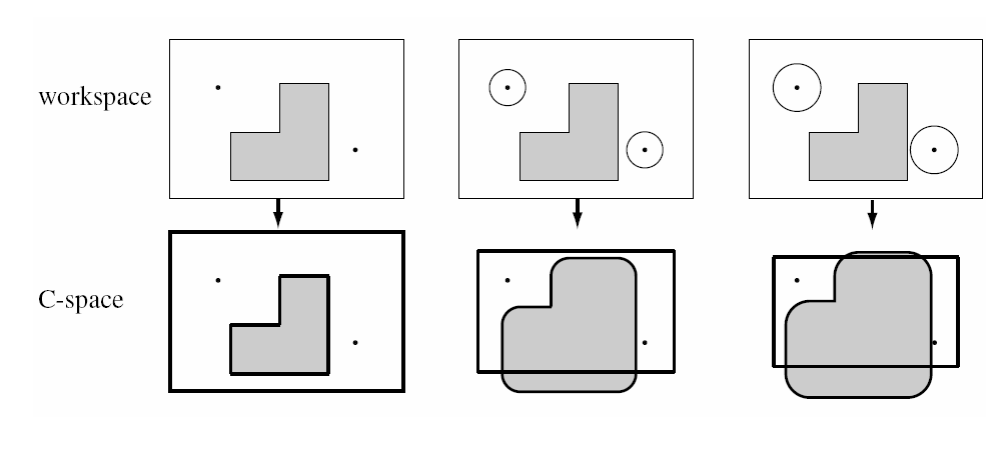
\includegraphics[width=12cm]{Figs/cspace_vs_workspace.png}
\par
\caption{\label{fig:cspace}Explicación gráfica en 2D de la diferencia entre el espacio de trabajo y el espacio de configuraciones.}
\end{figure}

Aplicado a nuestra práctica, el algoritmo consiste en comenzar a generar de forma simultánea un "árbol"  desde el inicio y el destino del movimiento. El árbol inicio se irá expandiendo por posiciones cercanas aleatorias que cumplan las distintas restricciones programadas, hasta que toque al árbol destino, que sigue el mismo patrón de comportamiento, en un determinado punto. En ese momento, se habrá encontrado una solución para la planificación, es decir, un camino válido entre la posición inicial y la final que debe poder ser ejecutado sin impedimentos (ver Figura \ref{fig:rrtConnect}). Nótese que cuanto más precisos sean los saltos hacia el siguiente punto del árbol, menor será la probabilidad de infringir zonas inválidas del espacio de configuraciones del robot. 



\begin{figure}[hbt!]
\centering
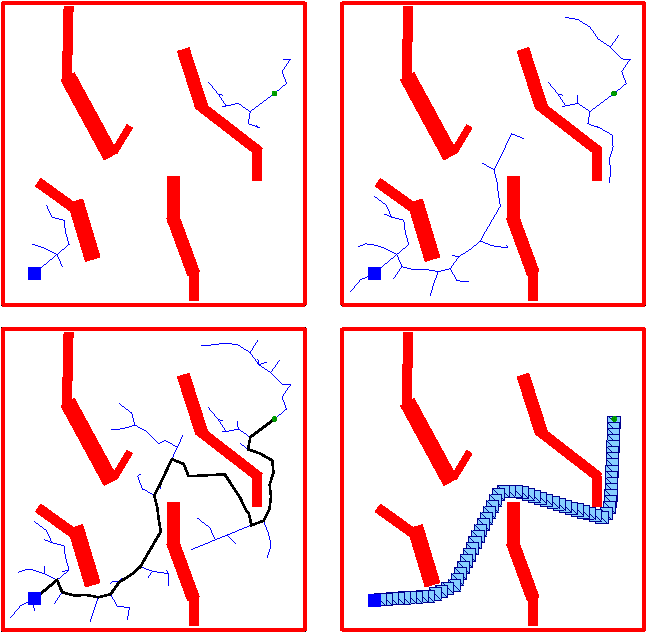
\includegraphics[width=12cm]{Figs/rrtConnect.png}
\par
\caption{\label{fig:rrtConnect}Explicación gráfica del algoritmo RRT Connect utilizado.}
\end{figure}

\section{Validación experimental}
Como se ha deslizado en los anteriores capítulos, la ejecución típica \footnote{Vídeo de ejemplo para la ejecución típica de la práctica con un objeto de color azul: https://youtu.be/OU1iNR0tzyA} \footnote{Vídeo de ejemplo para la ejecución típica de la práctica con un objeto de color rojo: https://youtu.be/Np2g\_3XHoH4} de la práctica requiere el lanzamiento de varios ficheros. En primer lugar, se debe ejecutar un comando \textit{source} que permita utilizar los paquetes personalizados por el desarrollador en su espacio de trabajo. Dicho comando podría añadirse al fichero \textit{.bashrc} para que se detecten los paquetes dentro del directorio creado cada vez que se arranque un terminal en Linux. El fragmento a escribir en línea de comandos sería: 
	\begin{lstlisting}[frame=single]
source ~/pr2_gazebo_tfg/devel/setup.bash
    \end{lstlisting}
    
A continuación se pueden ejecutar, en distintos terminales, los ficheros que cargarán el entorno Gazebo y el entorno de planificación. Posteriormente, se ejecuta la plantilla \textit{template.py} con la solución al ejercicio. Para ello, se requieren los siguientes comandos: 
\begin{itemize}
    \item Lanzar el mundo gazebo, que incluye el robot PR2 y sus modelos.
	\begin{lstlisting}[frame=single]
roslaunch pr2_gazebo tfg_launch.launch
    \end{lstlisting}
    \item Lanzar MoveIt! y las configuraciones de planificación necesarias para el robot PR2.
	\begin{lstlisting}[frame=single]
roslaunch pr2_moveit_config pr2_planning_execution_tfg.launch
    \end{lstlisting}
    \item Lanzar el script template.py.
	\begin{lstlisting}[frame=single]
rosrun moveit_tutorials template.py
    \end{lstlisting}
\end{itemize}
Una vez realizados los pasos anteriores, podremos observar en el simulador Gazebo la ejecución típica de la práctica de planificación y ejecución de trayectorias con MoveIt!, así como las imágenes del proceso descargadas en la máquina local. 
En primer lugar tiene lugar la fase 1, donde podemos observar al robot PR2 iniciando un movimiento de su cabeza hacia el lado derecho, apuntando la cámara Kinect hacia la zona de muestra (ver Figura \ref{fig:fase1}).

\begin{figure}[hbt!]
\centering
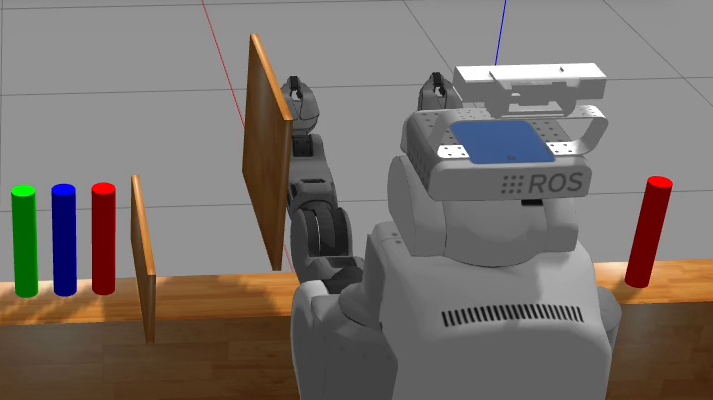
\includegraphics[width=7cm]{Figs/fase1_1.png}
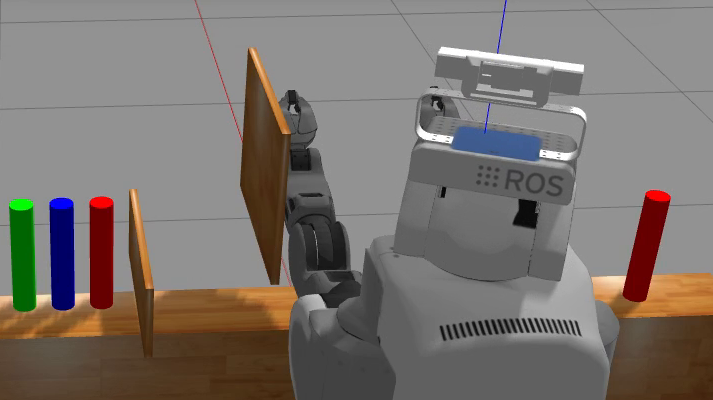
\includegraphics[width=7cm]{Figs/fase1_2.png}
\par
\centering
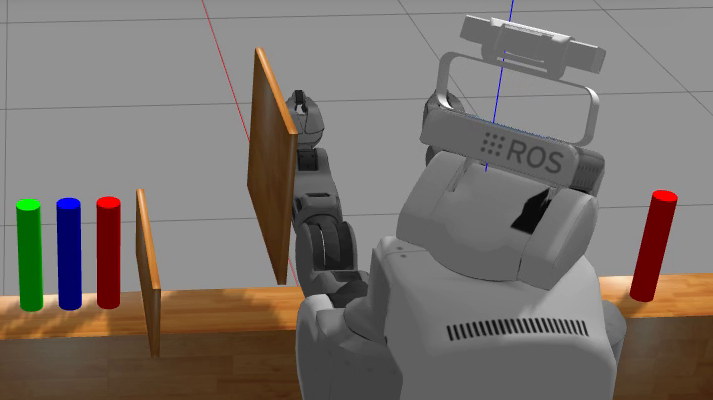
\includegraphics[width=7cm]{Figs/fase1_3.png}
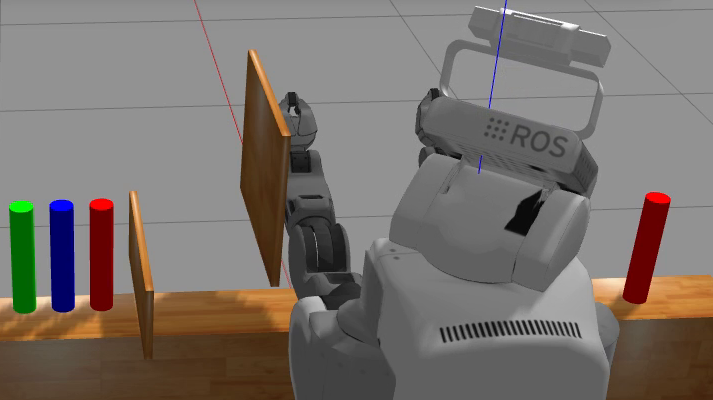
\includegraphics[width=7cm]{Figs/fase1_4.png}
\par
\caption{\label{fig:fase1}Secuencia de la fase 1 que muestra el movimiento de la cabeza del robot}
\end{figure}

A continuación se obtiene una imagen RGB a través de Kinect que se debe transformar al espacio HSV utilizando OpenCV para después aplicar las máscaras de color para el rojo, el verde y el azul. El funcionamiento del detector de objetos que ofrece la API de manejo de imágenes, permite detectar únicamente el color válido y descartar aquellos en los que se observa algo de ruido al aplicar la máscara de color, ya que de otra manera el robot detectaría objetos que en realidad no son válidos (ver Figura \ref{fig:fase2}).

\begin{figure}[hbt!]
\centering
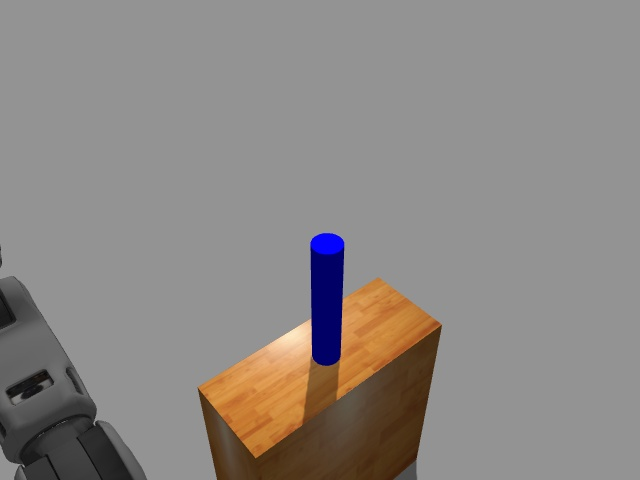
\includegraphics[width=7cm]{Figs/fase2_1.jpeg}
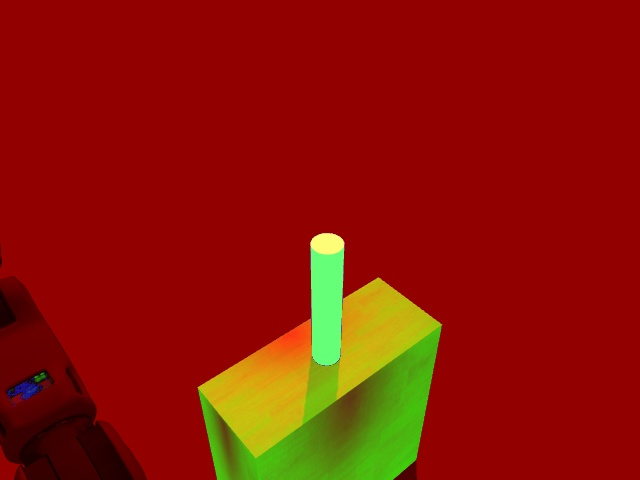
\includegraphics[width=7cm]{Figs/fase2_2.jpeg}
\par
\centering
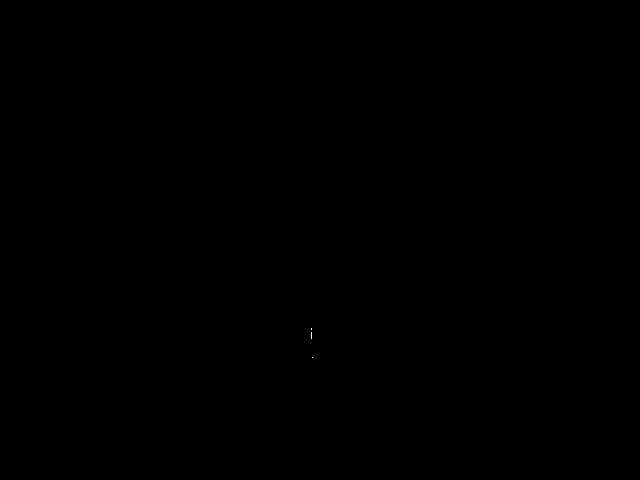
\includegraphics[width=4.66cm]{Figs/red_mask.jpeg}
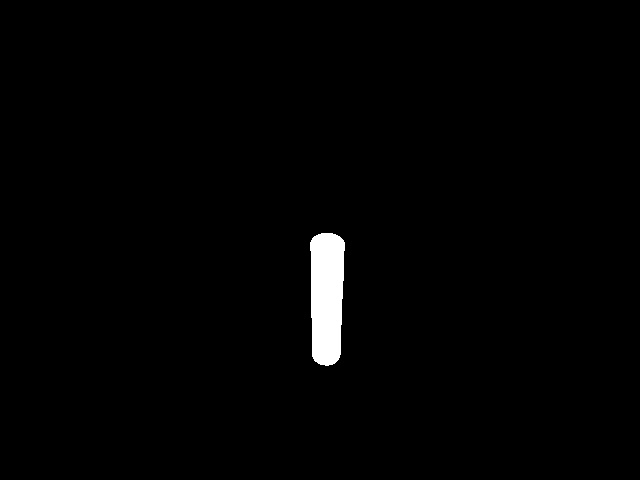
\includegraphics[width=4.66cm]{Figs/blue_mask.jpeg}
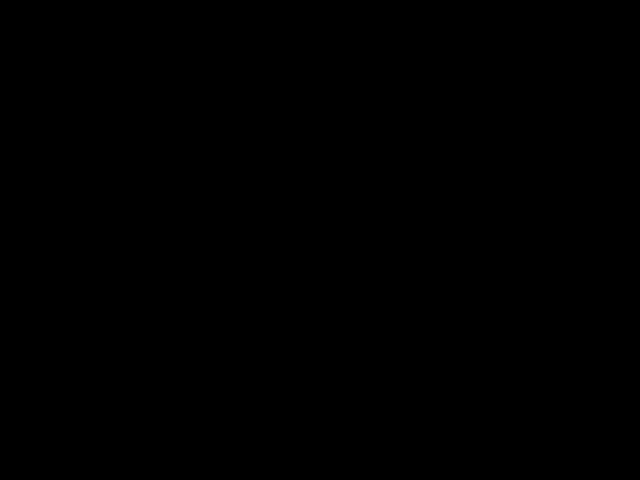
\includegraphics[width=4.66cm]{Figs/green_mask.jpeg}
\par
\caption{\label{fig:fase2}Secuencia de la fase 2 que muestra la transformación al espacio HSV y los resultados tras aplicar las máscaras de color para el rojo, azul y verde, respectivamente}
\end{figure}

Una vez conocido el color del objeto, y por tanto la posición destino a utilizar como meta del primer movimiento, se calcula una trayectoria hasta ella utilizando MoveIt!. Se realizarán entonces los dos trayectos en que se divide el movimiento. El primero de ellos es el más complejo, y consiste en pasar por debajo del primer obstáculo y por encima del segundo y situarse frente al objeto cuyo color coincida con el de la zona de muestra (ver Figura \ref{fig:fase4}). 

\begin{figure}[hbt!]
\centering
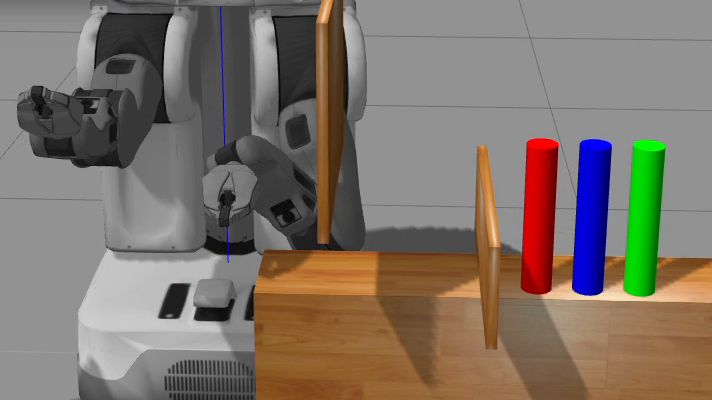
\includegraphics[width=7cm]{Figs/fase3_1.png}
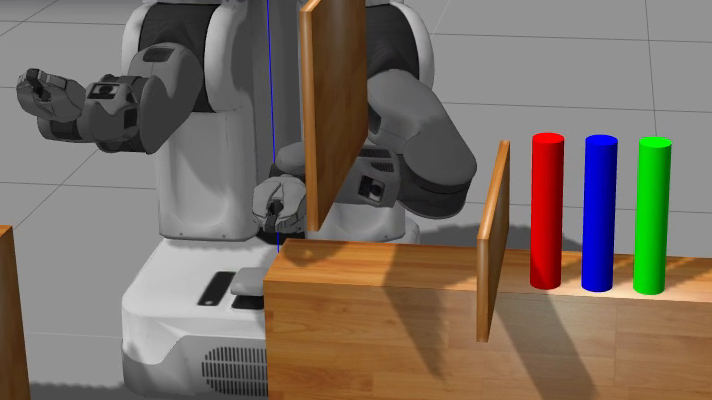
\includegraphics[width=7cm]{Figs/fase3_2.png}
\par
\centering
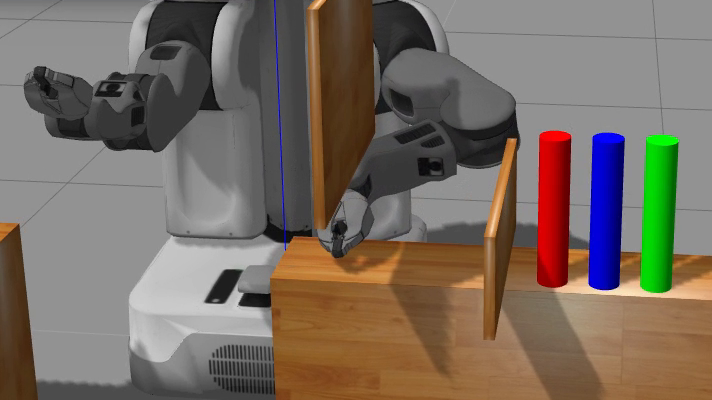
\includegraphics[width=7cm]{Figs/fase3_3.png}
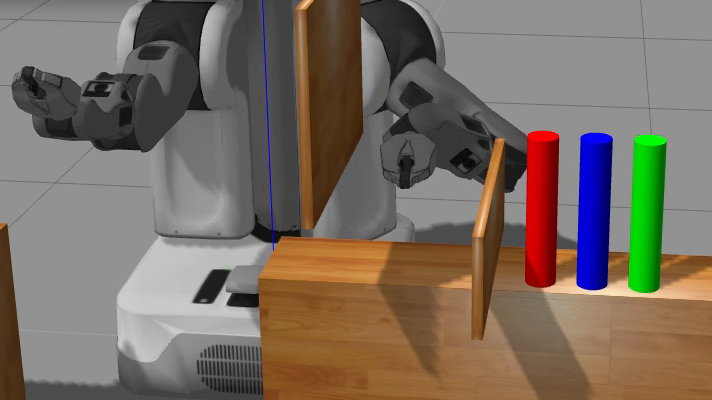
\includegraphics[width=7cm]{Figs/fase3_4.png}
\par
\centering
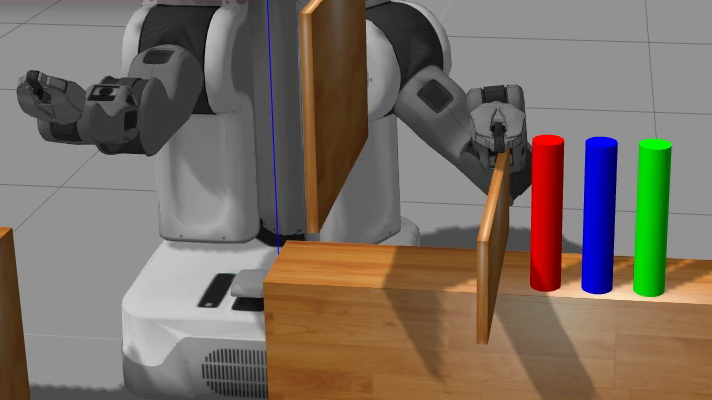
\includegraphics[width=7cm]{Figs/fase3_5.png}
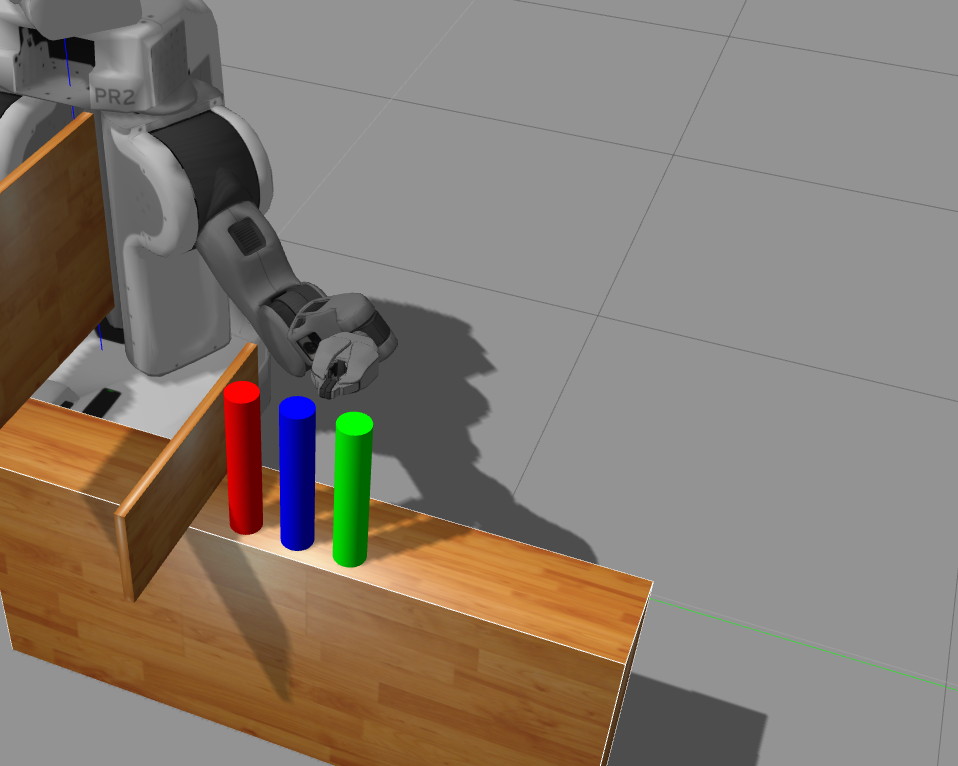
\includegraphics[width=7cm]{Figs/pos1_1.png}
\par
\caption{\label{fig:fase4}Secuencia de la fase 4 que muestra la ejecución de la trayectoria planificada en la fase 3}
\end{figure}

Por último, se puede observar el movimiento de derribo con el extremo del brazo izquierdo del robot, haciendo caer el objeto esperado y finalizando así la ejecución de la práctica (ver Figura \ref{fig:fase5}). 

\begin{figure}[hbt!]
\centering
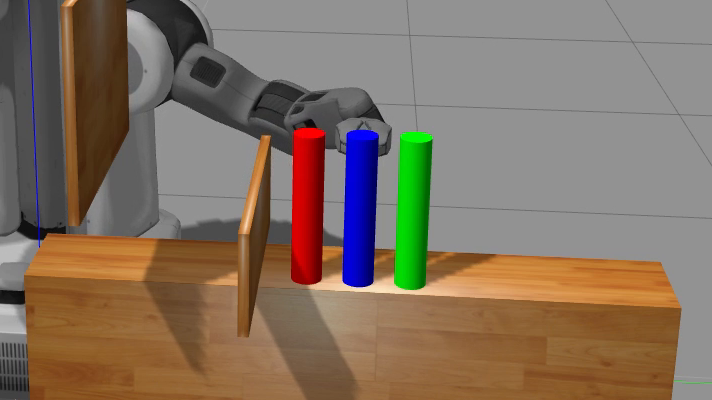
\includegraphics[width=7cm]{Figs/fase5_1.png}
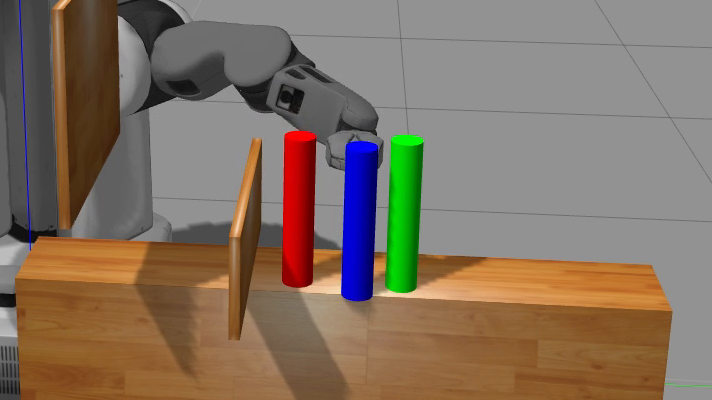
\includegraphics[width=7cm]{Figs/fase5_2.png}
\par
\centering
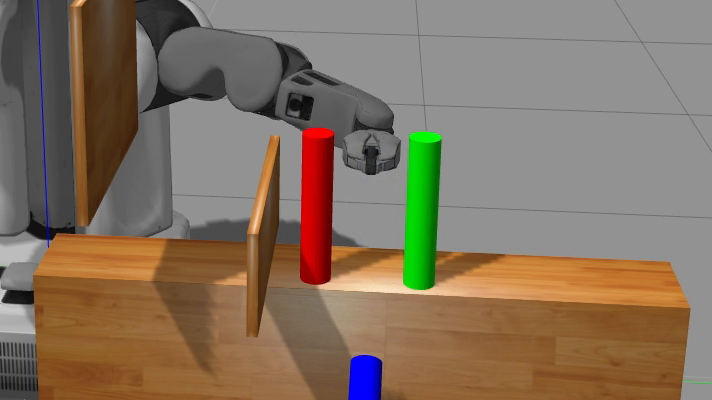
\includegraphics[width=7cm]{Figs/fase5_3.png}
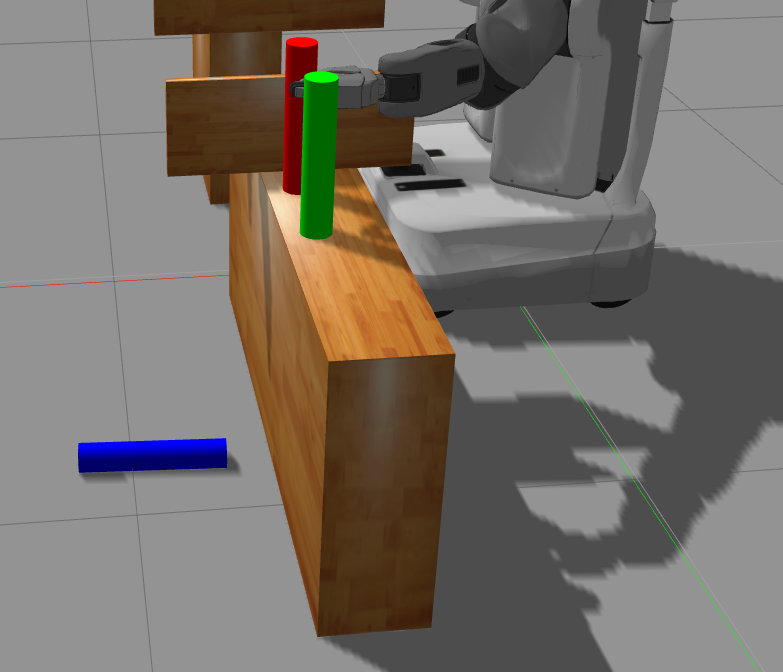
\includegraphics[width=7cm]{Figs/pose2_2.png}
\par
\caption{\label{fig:fase5}Secuencia de la fase 5 que muestra el movimiento de derribo}
\end{figure}

\section{Alternativas probadas}
\subsection{Ajuste del entorno}

Durante el desarrollo de la práctica ha sido necesario realizar pruebas con diferentes distancias entre el robot, los obstáculos, los objetos y las zonas. Todo ello en búsqueda de los límites del robot, una complejidad adecuada para la ruta de planificación entre los obstáculos del mundo (ver Figura \ref{fig:rviz}) o la distancia idónea para que el apartado visual y estético. 

\begin{figure}[hbt!]
\centering
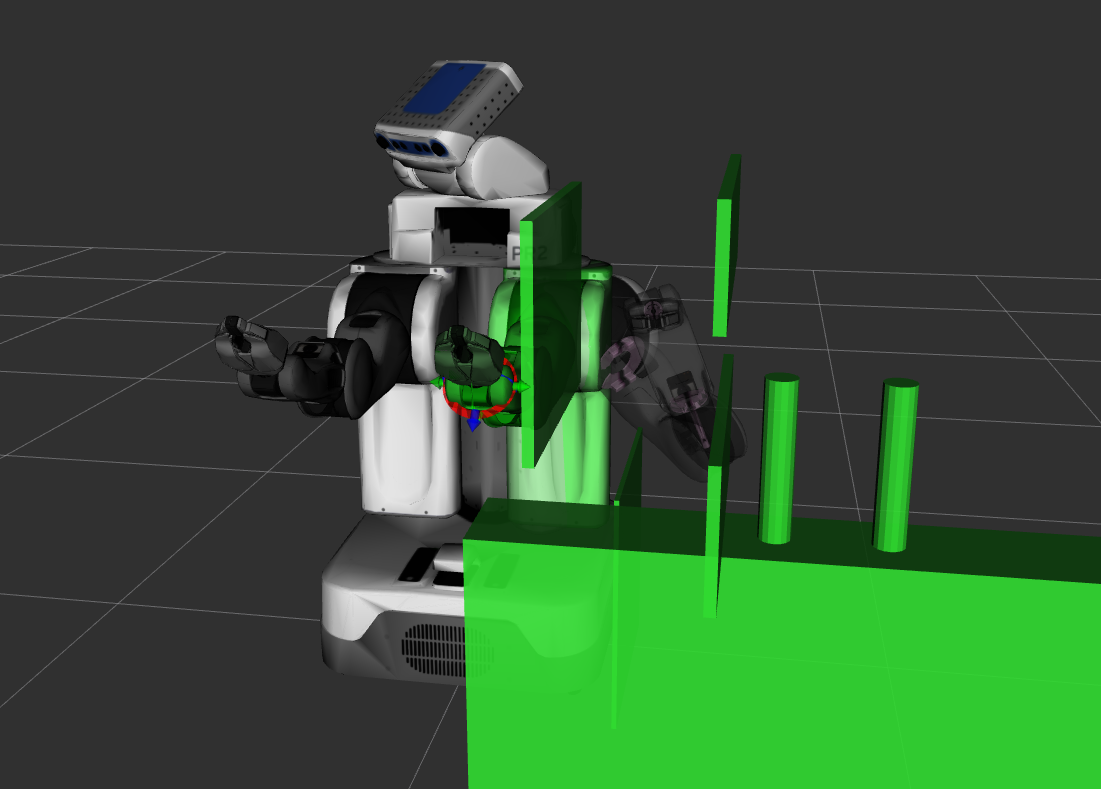
\includegraphics[height=6cm]{Figs/RVIZ.png}
\par
\caption{\label{fig:rviz}Situación creada dinámicamente en RVIZ durante las pruebas con obstáculos}
\end{figure}

Para llevar a cabo este ensayo se ha utilizado el visualizador RVIZ, una herramienta de MoveIt! que permite configurar los elementos del entorno sin necesidad de utilizar el simulador Gazebo, haciendo posible validar planificaciones secuencialmente sin reiniciar ningún proceso. Entre otras tareas permite planificar movimientos con las diferentes articulaciones del robot, visualizar información de los sensores a través d eun determinado topic, añadir objetos ficticios, realizar pruebas con diferentes configuraciones del planificador u obtener coordenadas en el espacio. 

Se ha generado un fichero llamado textit{pr2\_planning\_execution\_tfg\_rviz.launch} que permite lanzar el entorno de planificación incluyendo el visualizador, de manera que el desarrollador pueda probar nuevos escenarios o depurar sus cambios de forma sencilla. Para ello, es necesario añadir algunas líneas al fichero \textit{.launch} \cite{planning_rviz}.  %pending: renombrar dicho fichero en el repo
\vspace{20pt}
\begin{algorithm}[htb!]
	\begin{lstlisting}[breaklines=true,language=xml] 
<include file="$(find pr2_moveit_config)/launch/moveit_rviz.launch">
<arg name="config" value="true"/>
</include>
	\end{lstlisting}
\caption{\label{alg:planning_rviz}Líneas a añadir en el fichero de lanzamiento del entorno de planificación para incluir RVIZ.}
\end{algorithm}

\subsection{Ajuste del planificador}

La primera de las trayectorias ejecutadas por el brazo robótico del PR2 es la de mayor complejidad, trabajando con la planificación de trayectorias para esquivar varios obstáculos. En este punto ha sido necesario ajustar el parámetro del planificador OMPL llamado \textit{longest\_valid\_segment\_fraction}, que define la distancia a la que se considera asumible viajar por el espacio en búsqueda del siguiente nodo del grafo sin validar el estado de colisiones. Es decir, valores altos de este parámetro serán más rápidos pero podrían provocar errores en zonas estrechas o esquinas, y valores bajos garantizarán que el robot no se choque en su trayectoria a cambio de más lentitud. 

Entender como se calculan las posibles trayectorias en OMPL implica que el valor predeterminado por MoveIt! para este parámetro, que es configurable a través del fichero \textit{ompl\_planning.yaml} e igual a 0.05 por defecto, no tiene por qué ser el idóneo. Para adaptarlo a las necesidades de esta práctica ha sido necesario modificarlo, tras el análisis  realizado simulando 30 planificaciones para diferentes combinaciones según el número de obstáculos y la configuración de \textit{longest\_valid\_segment\_fraction}  (ver Figura \ref{fig:analisis_ejecuciones}).

\begin{figure}[hbt!]
\centering
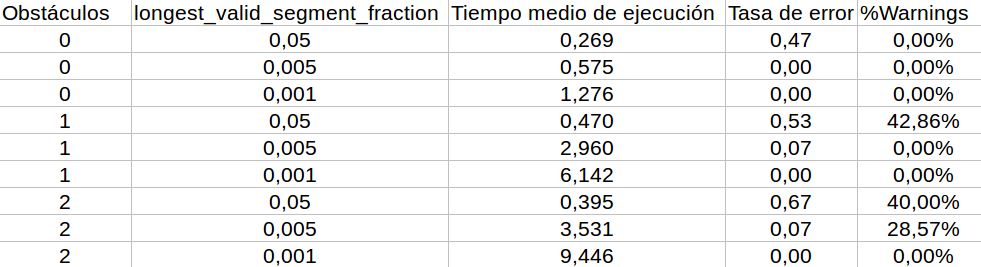
\includegraphics[width=14cm]{Figs/analisis_ejecuciones.png}
\par
\caption{\label{fig:analisis_ejecuciones}Respuesta del sistema ante distintas situaciones de entorno y diferentes configuraciones del planificador.}
\end{figure}

Como se puede observar, cuanto más complejo es el escenario, mayor precisión es necesaria para no obtener errores o \textit{warnings} en la planificación que pueden provocar problemas al ejecutar la ruta. En base a los resultados obtenidos, se ha decidido utilizar un valor de 0.001, ya que es el que garantiza un resultado fiable en el escenario final con 2 obstáculos. Por motivos de fiabilidad y optimización, el algoritmo calculará dos trayectorias y elegirá el mejor resultado, como se ha configurado a través del método \textit{set\_num\_planning\_attempts} que ofrece \textit{MoveGroupCommander}. 

\chapter{Conclusiones}
El capítulo final está enfocado a transmitir cuáles han sido los objetivos cumplidos satisfactoriamente, qué ha aportado el camino realizado para lograrlos, y qué líneas de trabajo se podrían seguir para mejorar o aprovechar los resultados de este Trabajo de Fin de Grado.  
\section{Conclusiones}

El objetivo formal propuesto al comienzo del desarrollo del proyecto ha sido alcanzado con éxito, generando una práctica completa de planificación de trayectorias utilizando herramientas modernas y extendidas en el ámbito robótico. Se logra así enriquecer el entorno educativo Robotics-Academy con el primer ejercicio sobre brazos robóticos disponible. 

El desarrollo de esta práctica ha supuesto importantes retos que enfrentar. En primer lugar, enfrentarse a un área de conocimiento nueva hasta ser capaz de aprovechar las posibilidades que ofrece y completar una solución técnica que incluye el habitual software heterogéneo de la robótica. Desde el nodo ROS creado se han integrado elementos que van desde la biblioteca de procesamiento de imágenes OpenCV hasta el entorno de planificación para robots MoveIt!.

El camino hasta la solución de referencia ha sido largo, con numerosas alternativas probadas. Estas dificultades han requerido aprender cada semana para resolver los problemas del día a día, mejorando así en una de las facetas clave de la ingeniería y adquiriendo nuevos conocimientos.

Finalmente, se ha creado la práctica "Movimiento planificado de un brazo robótico". Para ello se ha creado un mundo en Gazebo (ver sección \ref{sec:infraestructura}) que consiste en un robot PR2, dos zonas de acción, cilindros de colores y algunos obstáculos, que sirve como punto de partida para poder desarrollar el ejercicio de planificación. El modelo del robot PR2 ha requerido algunos cambios, como añadir por defecto una cámara Kinect sobre su cabeza o la desactivación del sensor láser para evitar problemas de ruido en las imágenes obtenidas por la cámara. 

Con el objetivo de ofrecer una plantilla en Python que simplifique el contacto con el procesamiento de imagen y la planificación con robots, se ha desarrollado un fichero \textit{template.py} que permite acceder a través de dos APIs a las funcionalidades relacionadas con cada uno de dichos procesos (ver sección \ref{sec:plantilla}). De esta manera, los alumnos pueden abstraerse de la complejidad de OpenCV y MoveIt! y preocuparse únicamente de obtener una solución válida, sin necesidad de configurar las transformaciones entre espacios de color, los umbrales de detección de contornos en imágenes, los controladores del PR2, los umbrales adecuados para el planificador RRT Connect o los ROS \textit{topics} utilizados para definir las posiciones objetivo de los distintos movimientos.

Por último, se ha desarrollado una solución de referencia (ver sección \ref{sec:solución}) a través del diseño de varias fases que dividen el problema a resolver. La primera de ellas consiste en actuar sobre los controladores de la cabeza del PR2 para lograr que gire a la derecha y observe la zona de muestra. A continuación, se utiliza la cámara Kinect para obtener una imagen que se transforma al espacio de color HSV con OpenCV y detecta si realmente hay un objeto y su color. Después, la interfaz de MoveIt! para Python \textit{moveit\_commander}  permite planificar y ejecutar una trayectoria con el brazo izquierdo del robot hasta situarlo frente al objeto a derribar, que será aquel cuyo color coincide con la zona de muestra. Por último, se realiza un movimiento de derribo que hace caer el cilindro.

Además del apartado puramente técnico, la motivación ha permitido superar el reto de completar un proyecto de ingeniería actual e innovador utilizando metodología de desarrollo de software ampliamente extendida. Ello ha permitido profundizar en habilidades útiles para el entorno laboral, como pueden ser ampliar los conocimientos de programación y tratamiento de imágenes, conocer el mundo de la robótica, diseñar modelos y arquitecturas, optimizar costes o trabajar en una solución integrada por distintos componentes que se comunican entre sí.  

\section{Trabajos futuros}

La solución aquí propuesta puede abrir la puerta a algunas líneas de trabajo futuras que, o bien supongan avances para la práctica realizada, o bien supongan nuevas prácticas que hagan uso de los conceptos y código desarrollados. 

Un primer avance podría ser hacer uso de las imágenes de profundidad ya aportadas por la cámara Kinect para calcular la posición relativa de los objetos en la zona destino, y utilizar dichas posiciones para calcular el destino de la planificación. Esta funcionalidad podría completarse calculando también la localización y tamaño de los obstaćulos y objetos para tenerlos en cuenta al planificar. 

Otra idea para profundizar en el uso de MoveIt!, sería añadir una tercera zona de acción en la que el robot deposite el objeto del color correspondiente, a través de maniobras de \textit{Pick and Place}. Para ello sería necesario aprender a manejar los mensajes y dispositivos de agarre, para lo que los tutoriales oficiales de MoveIt! pueden ser de gran ayuda.

Por último, podría ser conveniente adaptar el código a la nueva versión ROS2 \cite{ros2}, acompañada recientemente de la versión alfa de MoveIt!2 \cite{moveit2}. Ambas introducen mejoras importantes relacionadas con planificación, movimientos del robot y nueva funcionalidad. De manera análoga, igual que el robot PR2 se escogió por motivos de diseño y compatibilidad con ROS Kinetic, será requisito migrar la solución a un nuevo robot. Los nuevos lanzamientos incluyen el robot modular MARA \cite{mara}, de Acutronic Robotics, como el primer robot compatible.

Si el trabajo futuro se centrase en el estudio teórico o la obtención de métricas relacionadas con la planificación, una opción sería profundizar en los algoritmos de planificación disponibles en MoveIt! y comparar su rendimiento en distintas situaciones, o incluso generar los propios para controlar su funcionamiento en búsqueda del mayor beneficio. 

\printbibliography[heading=bibintoc]
\printindex

\end{document}
